%% The first command in your LaTeX source must be the \documentclass command.
\documentclass[sigplan,screen]{acmart}

\newif\ifdraft\drafttrue
%% Notes

\usepackage{xcolor}
\usepackage{xspace}

\definecolor{darkgreen}{RGB}{0,150,0}
\definecolor{darkorange}{RGB}{191,114,13}
\newcommand\todo[1]{\ifdraft\textcolor{red}{\textbf{TODO:} #1}\fi}
\newcommand\nv[1]{\ifdraft\textcolor{purple}{\textbf{NV:} #1}\fi}
\newcommand\mmg[1]{\ifdraft\textcolor{teal}{\textbf{MMG:} #1}\fi}
\newcommand\leo[1]{\ifdraft\textcolor{darkgreen}{\textbf{LEO:} #1}\fi}
\newcommand\hen[1]{\ifdraft\textcolor{darkorange}{\textbf{HENRY:} #1}\fi}

\newcommand{\cn}{\ifdraft\textsuperscript{\textcolor{blue}{[citation needed]}}\xspace\fi}

%% Text 
\newcommand\ie{{i.e.,}\xspace}
\newcommand\eg{{e.g.,}\xspace}
\newcommand\resp{{resp.}\xspace}

%% System names
\newcommand\Fstar{F${}^*$}

%% EDSL names
\newcommand{\LangA}{proof macro language\xspace}
\newcommand{\LangATerm}{proof macro\xspace}
\newcommand{\LangB}{proto-proof language\xspace}
\newcommand{\LangBTerm}{proto-proof term\xspace}

\newcommand{\TheTool}{the tool\xspace}

\usepackage{listings}

% uncomment next line to restore colors
\def\withcolor{}


\ifdefined\withcolor
  \definecolor{fstarblue}{rgb}{0.0, 0.0, 1.0}
  \definecolor{haskellstr}{rgb}{0.2, 0.2, 0.6}
  \definecolor{haskellred}{rgb}{1.0, 0.0, 0.0}
  \definecolor{gray_ulisses}{gray}{0.55}
  \definecolor{castanho_ulisses}{rgb}{0.59,0.42,0.15}
  \definecolor{preto_ulisses}{rgb}{0.55,0.28,0.59}
  \definecolor{green_ulises}{rgb}{0.59,0.42,0.15}
\else
	\definecolor{fstarblue}{gray}{0.1}
	\definecolor{haskellstr}{gray}{0.1}
	\definecolor{haskellred}{gray}{0.1}
	\definecolor{gray_ulisses}{gray}{0.1}
	\definecolor{castanho_ulisses}{gray}{0.1}
	\definecolor{preto_ulisses}{gray}{0.1}
	\definecolor{green_ulisses}{gray}{0.1}
\fi

\def\codesize{\small}

\lstdefinelanguage{HaskellUlisses} {
	basicstyle=\ttfamily\codesize,
	sensitive=true,
	%% morecomment=[s][\color{gray_ulisses}\ttfamily\itshape\codesize]{-}{-},
	%% morecomment=[l][\color{gray_ulisses}\ttfamily\itshape\codesize]{--},
	%% morecomment=[s][\color{gray_ulisses}\ttfamily\itshape\codesize]{\{-}{-\}},
	%% morecomment=[s][]{\{-@}{@-\}},
	morestring=[b]",
	stringstyle=\color{haskellstr},
	basewidth={0.53em},
	showstringspaces=false,
	numberstyle=\codesize,
	numberblanklines=true,
	showspaces=false,
	breaklines=true,
	showtabs=false,
	tabsize=4,
    literate={ {/\\}{{$\land$}}2
             {->}{{$\rightarrow$}}2
			 {<=>}{{$\Leftrightarrow$}}1
%			 {<=}{{$\leq$}}1
%			 {>=}{{$\geq$}}1
             {forall}{{$\forall$}}1
			 {'a}{{$\alpha$}}1
			 {labelty}{{$l$}}1
             {True}{{$\top$}}1
             {~int}{{$\mathbb{Z}$}}1
             {~nat}{{$\mathbb{N}$}}1
			 {==>}{{$\Longrightarrow$}}1
			 {=>}{{$\Rightarrow$}}1
			 {`feq`}{{$\eqinfix$}}1
			 {ka}{{k${}_a$}}1
			 {kb}{{k${}_b$}}1
			 {dollar}{{$\$$}}1
			 {dsl}{{d$_{sl}$}}2
			 {dfs}{{d$_{fs}$}}2
			 {rsl}{{r$_{sl}$}}2
			 {rfs}{{r$_{fs}$}}2
			 {dlm}{{d$_{lm}$}}2
           },
	emph=
	{[1] Set, Level, Axiom, Propositional, Extensionality, Tot, Type, bool, Lemma, ensures, requires, Ifc, IFC, IfcClearance, GlobalInt, GTot
	},
	emphstyle={[1]\color{fstarblue}},
	emph=
	{[2] class, match, with, if, then, else, let, rec, type, val, in, instance, data, measure, where, effect,noeq, private
	},
	emphstyle={[2]\color{castanho_ulisses}},
	emph=
	{[3]
        lattice, value, equals, canFlow, meet, join, bottom, top, 
        lawBot, lawFlowReflexivity, lawFlowAntisymetry, lawFlowTransitivity, 
        lawMeet, lawJoin, labels, 
        lt, lmeet, ljoin, lcanFlow, eq,
        labeled, labeledTCB
	},
	emphstyle={[3]\color{preto_ulisses}\textbf},
	emph=
	{[4]
        Low, Medium, High
	},
	emphstyle={[4]\color{green_ulises}\textbf},
	emph=
	{[5] assume, admit, admitP
	},
	emphstyle=[5]\color{red}\textbf,%\underline, % underline not working
	% this emp 6 is a ban rule => highlight bad code
	emph={[6] leq, equals, join', c_0, c_1
	},
	emphstyle=[6]\color{green}\textbf,
}

\newcommand{\LC}{\lstinline[language=HaskellUlisses, basicstyle=\ttfamily]}

\lstnewenvironment{code}
{\lstset{language=HaskellUlisses}}
{}

\lstnewenvironment{scode}
{\lstset{language=HaskellUlisses,basicstyle=\ttfamily\footnotesize,keepspaces,mathescape}}
{}


\lstnewenvironment{mcode}
{\lstset{language=HaskellUlisses,columns=fullflexible,keepspaces,mathescape}}
{}

\lstnewenvironment{ccode}
{\lstset{language=C,columns=fullflexible,keepspaces,mathescape}}
{}

\lstMakeShortInline[language=HaskellUlisses,mathescape,keepspaces,mathescape,basicstyle=\ttfamily\codesize,breakatwhitespace]|


\usepackage[inference]{semantic}

\newcommand{\Rho}{\mathrm{P}}
\newcommand{\macroHole}[2]{\Box_{#1 ; #2}}
\newcommand{\expandsTo}{\rightsquigarrow}

\newcommand{\Expand}[4]{#1; #2 \vdash #3 \expandsTo #4}
\newcommand{\Interp}[2]{\llbracket #1 \rrbracket (#2)}
\newcommand{\Sem}[3]{\Interp{#1}{#2} = #3}

%% Rights management information.  This information is sent to you
%% when you complete the rights form.  These commands have SAMPLE
%% values in them; it is your responsibility as an author to replace
%% the commands and values with those provided to you when you
%% complete the rights form.
\setcopyright{none}
\copyrightyear{2018}
\acmYear{2018}
\acmDOI{XXXXXXX.XXXXXXX}

%% These commands are for a PROCEEDINGS abstract or paper.
% \acmConference[Conference acronym 'XX]{Make sure to enter the correct
%   conference title from your rights confirmation emai}{June 03--05,
%   2018}{Woodstock, NY}
% \acmPrice{15.00}
% \acmISBN{978-1-4503-XXXX-X/18/06}

%%
%% The majority of ACM publications use numbered citations and
%% references.  The command \citestyle{authoryear} switches to the
%% "author year" style.
%%\citestyle{acmauthoryear}

\begin{document}

\title{Liquid Proof Macros}

\author{Henry Blanchette}
\email{blancheh@umd.edu}
\affiliation{%
  \institution{University of Maryland}
  \city{College Park}
  \country{USA}
}
%\orcid{1234-5678-9012}

\author{Niki Vazou}
\email{niki.vazou@imdea.org}
\affiliation{%
  \institution{IMDEA}
  \city{Madrid}
  \country{Spain}
}

\author{Leonidas Lampropoulos}
\email{leonidas@umd.edu}
\affiliation{%
  \institution{University of Maryland}
  \city{College Park}
  \country{USA}
}

%%
%% By default, the full list of authors will be used in the page
%% headers. Often, this list is too long, and will overlap
%% other information printed in the page headers. This command allows
%% the author to define a more concise list
%% of authors' names for this purpose.
\renewcommand{\shortauthors}{Blanchette et al.}

%%
%% The abstract is a short summary of the work to be presented in the
%% article.
\begin{abstract}
Liquid Haskell is a popular verifier for Haskell programs,
leveraging the power of SMT solvers to ease users' burden of proof.
%
However, this reliance on SMT does not come without a price:
convincing the Liquid Haskell typechecker that a program is correct
often necessitates giving hints to the underlying solver, which can be
a tedious and verbose process that sometimes requires intricate
knowledge of Liquid Haskell's inner workings.

In this paper, we present {\em Liquid Proof Macros}, an extensible
metaprogramming technique and framework for simplifying the
development of Liquid Haskell proofs.
%
We describe how to leverage Template Haskell 
to generate Liquid Haskell proof terms, via a tactic-inspired DSL interface for
more concise and user-friendly proofs, 
%
and we demonstrate the capabilities of this framework by automating
a wide variety of proofs from an existing Liquid Haskell benchmark.
\end{abstract}

%%
%% The code below is generated by the tool at http://dl.acm.org/ccs.cfm.
%% Please copy and paste the code instead of the example below.
%%
\begin{CCSXML}
<ccs2012>
   <concept>
       <concept_id>10011007.10011074.10011099.10011692</concept_id>
       <concept_desc>Software and its engineering~Formal software verification</concept_desc>
       <concept_significance>500</concept_significance>
       </concept>
 </ccs2012>
\end{CCSXML}

\ccsdesc[500]{Software and its engineering~Formal software verification}

%%
%% Keywords. The author(s) should pick words that accurately describe
%% the work being presented. Separate the keywords with commas.
\keywords{Liquid Haskell, proof macros, tactics}

%%
%% This command processes the author and affiliation and title
%% information and builds the first part of the formatted document.
\maketitle

\section{Introduction}

Liquid Haskell~\cite{liquidHaskell} is a popular verifier for Haskell
programs, leveraging the power of SMT solvers~\cite{BarST-RR-10} (such
as Z3~\cite{Z3} or CVC4~\cite{CVC4}) to prove the correctness of
diverse applications ranging from optimizations~\cite{TPE2018} to
string matching algorithms~\cite{TaleOfTwoProvers}. Specifications for
these applications are written in the form of {\em refinement
  types}~\cite{RefinementForML}, boolean predicates over program
values.

For concreteness, consider the following \LC{min} function that
computes the minimum of two natural numbers, defined inductively:
\begin{code}
  data N = Z | S N
  
  min :: N -> N -> N 
  min Z _ = Z
  min _ Z = Z
  min (S m) (S n) = S (min m n)
\end{code}

\newcommand{\imin}{\textit{min}~}
Naturally, we would expect such a function to be associative, that is:
$$ \forall a ~ b ~ c. ~ \imin (\imin a~b)~c == \imin a~(\imin~b~c) $$
%
In Liquid Haskell, we can {\em specify} associativity by defining a
refinement type to encode this property, and we can {\em prove}
associativity by defining a term of that type:
%
\begin{code}
  {-@ assocMin :: a:N -> b:N -> c:N ->
      {_:() | min (min a b) c == min a (min b c)}
  @-}
  assocMin :: N -> N -> N -> Proof
  assocMin = ...
\end{code}
%
To Haskell, the type of \LC{assocMin} is simply a function with three
natural number arguments that returns a \LC{Proof}, which is just a
type synonym for \LC{()}. To Liquid Haskell, however, the type of
\LC{assocMin} is much more interesting: its return type does not only
specify that the output is a unit, but {\em refines} it so that
associativity of \LC{min} holds for its input arguments. In other
words, the only interesting thing about the result of this function is
its refinement, which constitutes an ``extrinsic style'' proof of
associativity. This is a common enough pattern that Liquid Haskell
supports dropping the ``\LC{_:()}'' part of the refinement for
brevity, as we will also do in the remainder of this paper.

But how does Liquid Haskell decide if the refinement type is true? By
reducing typechecking to verification conditions that SMT solvers
reason about. However, while SMT solvers are pre-programmed with a
wide assortment of facts about various domains such as integer
arithmetic and boolean logic, they don't really know anything about
user-defined data types like \LC{N} or user-defined functions like
\LC{min}. While a direct encoding of such features to SMT is possible
in principle~\cite{HALO}, it leads to unpredictable verification, also
known as the ``butterfly effect''~\cite{LeinoP16}. To that end, Liquid
Haskell lifts user-defined data types and functions into a
representation that can be handled symbolically by SMT
solvers~\cite{VazouTCSNWJ18}. Still, many true properties of
user-defined data types and functions remain not automatically
verifiable: users must guide, via refined Haskell code, the SMT solver
to simpler cases that can be checked automatically.

Unfortunately, given the lack of interactivity of Liquid Haskell, it
is not always clear what the gap in understanding between the user and
the SMT solver is, which often makes writing such refined code a
tedious and frustrating process. Consider again associativity for the
\LC{min} function. On paper, we can informally reason that
associativity holds by induction on the natural numbers that are inputs
to \LC{min}, due to its simple recursive structure. In Liquid Haskell,
the refined code that finally convinces the SMT solver that the
program typechecks is shown in Figure~\ref{fig:assoc-min-proof}.


% The SMT solver, however, does not know about induction (unlike Coq where a tactic "induction" could solve this goal right away).
% And, because of Liquid Haskell's limited capabilities for quantifying over predicates (TODO: include reference here), it is unfeasible to write the induction principle for natural numbers as a refined Haskell function.
% So, a proof of "assoc\_min" is written as follows:
\begin{figure}
\begin{code}
  {-@ assocMin :: a:N -> b:N -> c:N ->
        {min (min a b) c == min a (min b c)} @-}
  assocMin :: N -> N -> N -> Proof
  assocMin = \a b c ->
    case a of 
      Z ->
        case b of 
          Z ->
            case c of
              Z -> trivial
              S c' -> trivial
          S b' ->
            case c of
              Z -> trivial
              S c' -> trivial
    S a' ->
      case b of 
        Z ->
          case c of
            Z -> trivial
            S c' -> trivial
        S b' ->
          case c of
            Z -> trivial
            S c' -> assocMin a' b' c'
\end{code}
\caption{Liquid Haskell proof term for associativity of \texttt{min}}
\label{fig:assoc-min-proof}
\end{figure}

{\em All} of the branches of pattern matching on \LC{a}, \LC{b}, and
\LC{c} must be written out explicitly. Otherwise, the SMT solver would
not know how to simplify the \LC{min} expressions in the
refinement---the only facts it knows are the three equations that were
used in \LC{min}'s definition:
%
\LC{min Z _ = Z}, \LC{min _ Z = Z}, and
%
\LC{min (S x) (S y) = S (min x y)}.
%
Liquid Haskell understands the constraints introduced by pattern
matching, and takes them into account in order to discharge most
cases---the non-recursive ones that involve at least one \LC{Z}. The
proof conclusion in such cases is \LC{trivial}, which is again just a
synonym for the term-level \LC{()}.

However, in the recursive case of \LC{min}, the Liquid Haskell typechecker needs
additional help, in the form of a recursive call to \LC{assocMin a' b' c'}, which
brings its refinement in scope for the SMT solver and allows it to conclude that
the induced verification condition holds. Crucially, this refinement is again the
only thing that matters: while the structure of the term gives the appearance
of a proof term in the style of Coq or Agda, the actual return value doesn't matter.
We could just as well have written something like
\begin{code}
  snd (assocMin a' b' c', ())
\end{code}
and Liquid Haskell would still gladly accept the definition. In fact,
Liquid Haskell's conjunction operator (\LC{&&&}) is defined exactly
this way: it takes two \LC{Proof}s and returns the second one---its
only effect is making the refinement of both arguments visible to the SMT solver.

Even in this simple example of associativity of \LC{min}, the full
verbosity required is cumbersome and obscures the fact that the
underlying argument is a straightforward induction. In larger
developments where the SMT solver might need to rely on helper lemmas,
this problem only becomes more pronounced.  Other proof assistants,
such as Coq~\cite{Coq}, Lean~\cite{Lean4}, or
Isabelle~\cite{Isabelle}, rely on interactive tactics in these
situations to aid users' proof efforts. But developers of these tactic
languages enjoy a transparent API to interact with the current proof
state, and an essentially clean slate to design metaprogramming
capabilities, which has been exploited to the great benefit of proof
assistant users~\cite{Ltac, Mtac, ltac2}.

On the other hand, Liquid Haskell interacts with the SMT solver in a
very opaque manner, and within the Haskell ecosystem metaprogramming
capabilities are already well established in the form of Template
Haskell---but not really designed with SMT-based verification in
mind. So then, {\em what can we do within the confines of this mature
  Haskell ecosystem to aid users?}  Without interactivity, an
interface to concise proof generators must expand to a proof term all
at once i.e. it must behave like a macro. Therefore, we developed a
macro system for generating Liquid Haskell proof terms, using the
existing metaprogramming tools for Haskell.
  % TODO: any other limitations to mention, that directed us to this solution?

\paragraph*{Liquid Proof Macros}

In this paper, we show how to leverage the power of Template Haskell
to automate proof term generation for Liquid Haskell.  We develop {\em
  Liquid Proof Macros}, an extensible DSL in which users can write
intutive proofs that resemble automated tactics%
\footnote{We refrain calling our DSL tactics in this paper, as that suggests a
  notion of interactivity that is impossible in the current version of Liquid
  Haskell. In truth, they lie somewhere between tactics (no interactivity)
  and macros (users have to dive into Template Haskell to extend the DSL).
}%
%
 of more traditional proof assistants, including case analysis,
 induction, conditioning, and proof search. For example, the same
 proof of associativity of \LC{min} using Liquid Proof macros can be
 seen in Figure~\ref{fig:assoc-min-macro}. 

These macros are expanded to a subset of Haskell that resembles, or
rather is even more complicated than, the one used in
Figure~\ref{fig:assoc-min-proof}. To facilitate typechecking of larger
Liquid Haskell developments, we also augment this subset with metadata
information, and provide a pruning algorithm reminiscent of shrinking
in property-based testing~\cite{ClaessenH00}, simplifying away any
unnecessary components that result from proof search. Section
\ref{sec:prune} details how our system defines and handles pruning.


\begin{figure}[t]
\begin{code}
  {-@ assocMin :: a:N -> b:N -> c:N ->
        {min (min a b) c == min a (min b c)} @-}
  [tactic|
    assocMin :: N -> N -> N -> Proof
    assocMin a b c = induct a; induct b; induct c
  |]
\end{code}
\caption{Associativity of \texttt{min} using Liquid Proof Macros}
\label{fig:assoc-min-macro}
\end{figure}

\pagebreak
In this paper we make the following contributions:
\begin{itemize}
\item We describe a methodology for using Template Haskell to
  automatically construct Liquid Haskell proof terms, and we develop
  an extensible framework using this methodology for automating
  inductive proofs in Liquid Haskell
  (Section~\ref{sec:liquid-proof-macros}).
\item We evaluate our framework against an existing benchmark
  containing a wide variety of Liquid Haskell properties, and found
  that our Liquid Proof Macros can be used to automate all of these
  properties, leading to a $1.57\times$ reduction in code on average
  (Section~\ref{sec:eval})
\end{itemize}
We then discuss related work (Section~\ref{sec:related}), before
concluding with a discussion of the limitations of our framework and
directions for future work (Section ~\ref{sec:future}).


\section{Implementation}

The proof macro system involves two stages:
- preprocessing:
  - preprocess EDSL into augmented subset of Haskell
  - embed augmented subset of Haskell into Haskell
- pruning:
  - pruning algorithm over augmented subset of Haskell 
    - augmentation keeps track of pruning-relevant metadata e.g. which terms have been prune/kept from an auto site
    - in each step of the pruning algorithm, checks if current prune is valid by embedding the current pruned expression into Haskell then running Liquid Haskell

\subsection{Preprocessing}

The proof macro is written by the user in an ESDL that appears inside a Haskell quasiquotation.
The EDSL has the following syntax:
\begin{align*}
  \textit{decl}~ ::= &
    \textit{name} ~ : ~ \textit{type} \\ &
    \textit{name} ~ \overline{\textit{name}} ~ = ~ \overline{\textit{instr} ; }
  \\
  \textit{instr} ~ ::= &
    \textbf{intro} ~ \textit{name} \\ | &
    \textbf{destruct} ~ \textit{name} ~ (\textbf{as} ~ \textit{destruct-pat}) ([\overline{\textit{flag},}]) \\ | &
    \textbf{induct} ~ \textit{name} ~ (\textbf{as} ~ \textit{pat}) ([\overline{\textit{induct-flag},}]) \\ | &
    \textbf{auto} ~ (\overline{\textit{name},}) (\textit{nat}) \\ | &
    \textbf{condition} ~ \textit{exp} ~ (\textbf{requires} ~ [\overline{\textit{name},}]) \\ | &
    \textbf{assert} ~ \textit{exp} ~ (\textbf{requires} ~ [\overline{\textit{name},}]) \\ | &
    \textbf{dismiss} ~ \textit{exp} ~ (\textbf{requires} ~ [\overline{\textit{name},}]) \\ | &
    \textbf{use} ~ \textit{exp} ~ (\textbf{requires} ~ [\overline{\textit{name},}]) \\ | &
    \textbf{trivial}
\end{align*}

The above proof macro ESDL is preprocessed into an augmented subset of Haskell. 
The particular subset is exactly the image of the EDSL preprocessor.
The conceptual distinction between the ESDL and the augmented substet is that preprocessing the EDSL requires a context and producing many expressions per single EDSL instruction. 
The augmented subset 

\subsection{Pruning}

\section{Design, Evaluation, and Usage}
\label{sec:eval}

In this section, we focus on the choices that influenced our design
(Section~\ref{sec:design}), we evaluate these choices in an existing
Liquid Haskell benchmark of programs (Section~\ref{sec:eval-eval}),
and demonstrate the usage of our tool with a small example
(Section~\ref{sec:example}).

\subsection{Design Choices}
\label{sec:design}

\begin{figure*}
  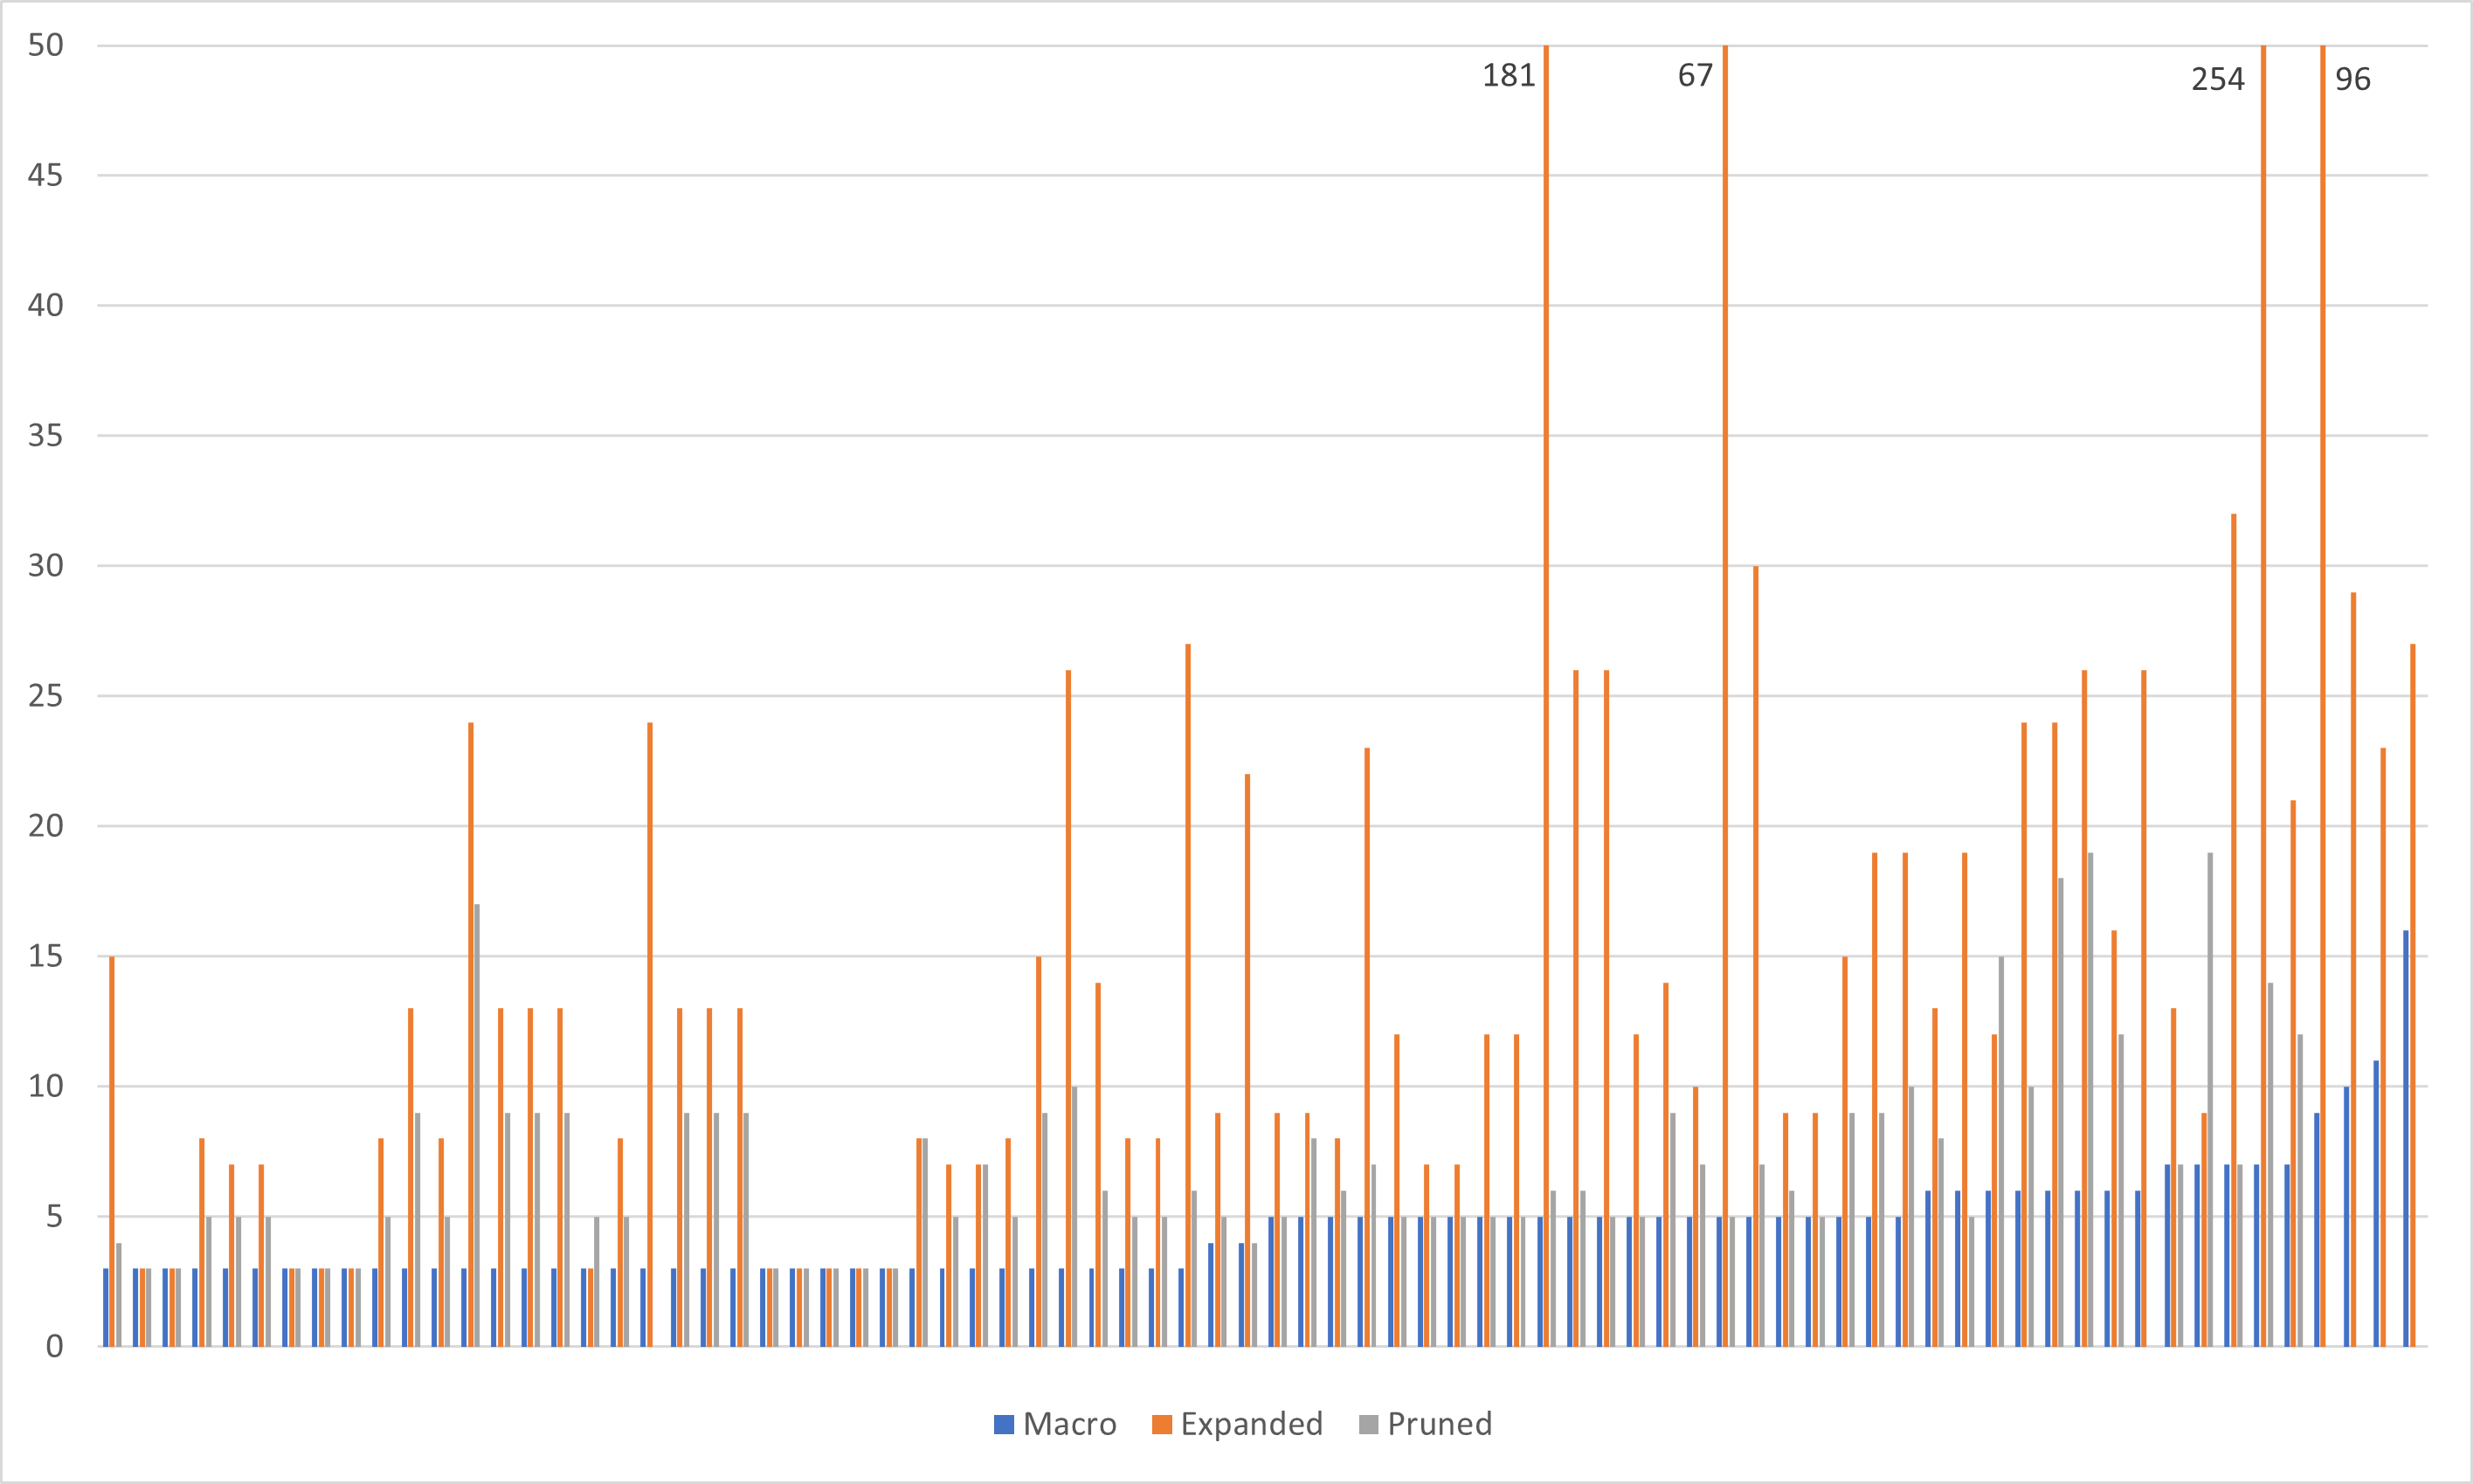
\includegraphics[width=\textwidth]{LiquidProofEval.png}
  \caption{LoC across benchmarks of Liquid Proof Macros (in \textcolor{blue}{blue}), the expanded splice (in \textcolor{orange}{orange}), and the minimal
    Liquid Haskell proof term (in \textcolor{gray}{gray})}
  \label{fig:loc-eval}
\end{figure*}

% % ? BEGIN OUTLINE

% The benefits we aim to provide with these proof macros are:
% - conciseness: the macros cater towards a specific subset of LH that is used
%   for extrinsic-style proofs, so the interface to this subset can be more
%   specific and restricted than generic programs
% - reduced redundancy: often, multiple logical branchings can be handled by the
%   same proof macro (due to the modularity the macros achieve in a similar
%   style to tactics), and proof macro branchings (such as destruct, induct,
%   condition) allow the handling proof macro to be written just once and then
%   used in all of the branches
% - modularity: in the same style as tactics, the auto proof macro is contextual
%   and so the same use of auto can be used to solve many different proof goals
%   by leveraging contextual information such as the lemmas, variables, and
%   sound recursions.

% To verify the applicability of these benefits, we selected an
% independently-curated collection of properties to be proved in an extrinsic
% style using Liquid Haskell: https://github.com/mustafahafidi/qc-to-lh. The
% original use of these properties was to demonstrate the usefulness of another
% approach to generating Liquid Haskell proofs that has some similarities to our
% approach.

% TODO: describe similarities and differences The properties are relatively
% basic properties about the natural numbers, lists of natural numbers or pairs
% of natural numbers, and trees of natural numbers.

% % ? END OUTLINE

When designing Liquid Proof Macros, we wanted users to benefit along the following three axis:

\paragraph{Conciseness.}
%
Extrinsic proofs are mostly written in a particular subset of Haskell,
the \LangB. Using metaprogramming to generate terms in this subset we
would expect proofs to be shorter than when written out explicitly.
%
%\paragraph{Reduced redundancy.}
%
Moreover, as most proof assistant users are familiar with, often many
different branches of a proof can be handled by the same proof
strategy. Rather than requiring users to replicate the same proof term
in each branch, proof macros allow for writing such strategies once
and applying them across all branches.

\paragraph{Modularity.}
%
Even though many proofs can be encapsulated by the same proof strategy
(e.g. simple induction), vanilla Liquid Haskell requires that strategy
to be written out in full verbosity in each instance (e.g.  pattern
matching on a list of a natural numbers, and then supplying the tail
or predecessor to the recursive call in the second cases
respectively). The proof macro system allows the user to modularly
encode proof strategies in such a way that the same sequence of proof
macros can be used to prove a wide variety of similar theorems that
use the same proof strategy.

\paragraph{Practicality}
%
The style of proof search used by our proof macro system is very
inefficient, verily because it includes all generatable neutral forms
(using a limited) context without using any sort of guided search. The
secondary pruning process, which is performed on a passing proto-proof
term after proof search is complete, aims to recover a minimal proof
term for the sake of readability and efficient re-checking.

\subsection{Evaluation}
\label{sec:eval-eval}

To evaluate our design, we turned to a prior benchmark suite of 80+
Liquid Haskell proofs~\cite{TacticThesis}, that consists of a
collection of boolean predicates over natural numbers, lists, and
binary trees, ranging from very simple facts to inductive properties
that require auxiliary lemmas. All proofs take advantage of both proof
macros, and {\em proof by logical evaluation}~\cite{VazouTCSNWJ18}, a
complementary technique for delegating some equational reasoning to
the SMT solver.

Using Liquid Proof Macros we were able to concisely prove ($<16$ LoC
for all and $<10$ LoC for all but two). Figure~\ref{fig:loc-eval}
shows the lines of code across all such benchmark using (1) Liquid
Proof Macros (2) the expanded proof term (3) the pruned minimal proof
term. We found that in all cases proof macros where smaller than the
Liquid Haskell proof terms, with a (geometric) average of 57\%
reduction in LoC compared to the minimal pruned version. Moreover, to
give an estimate of the cost of proof search, the unpruned expanded
splice generated by Template Haskell was $2.88\times$ larger on
average.

\subsection{Usage Example}
\label{sec:example}

% TODO: put screenshots here

\begin{figure*}
  \centering

  \begin{subfigure}[t][][t]{1\textwidth}
    % \centering
    \begin{minipage}[c]{0.5\textwidth}
      \caption{The user writes the proof macros.}
    \end{minipage}
    \hfill
    \begin{minipage}[c]{0.49\textwidth}
      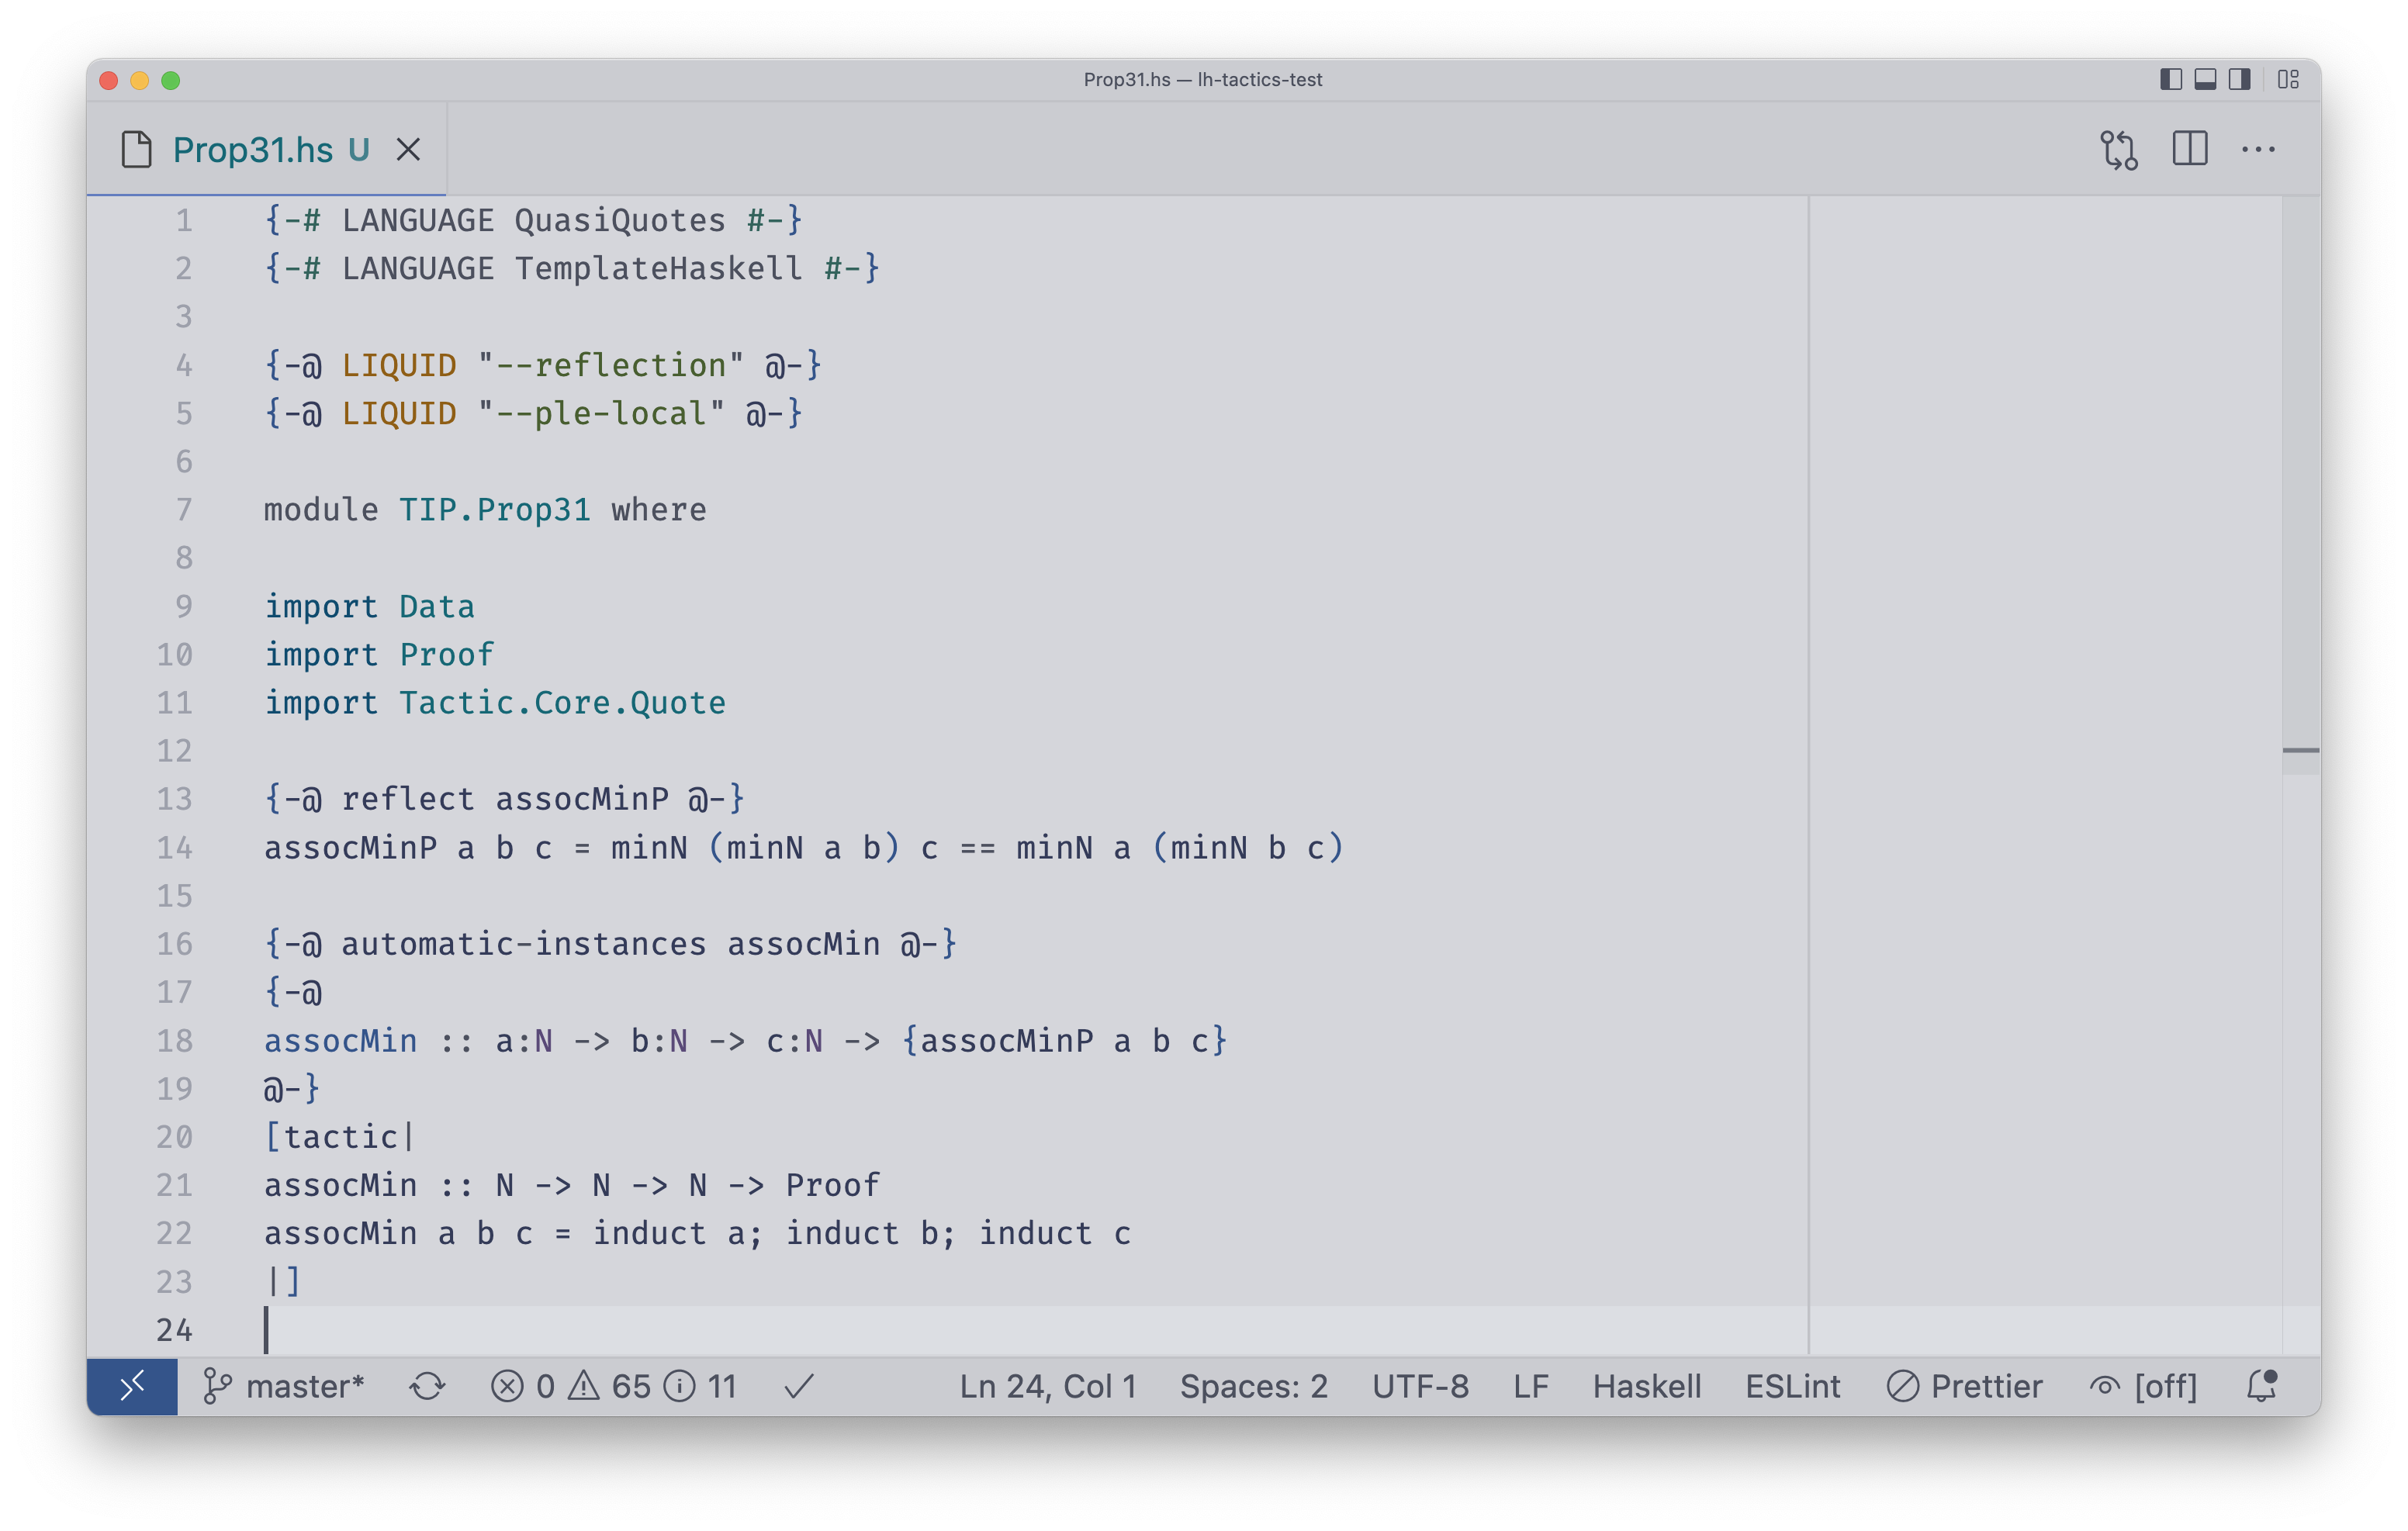
\includegraphics[width=\textwidth]{example-screenshots/macros.png}
    \end{minipage}
  \end{subfigure}
  \begin{subfigure}[t][][t]{1\textwidth}
    % \centering
    \begin{minipage}[c]{0.5\textwidth}
      \caption{The user runs the \LC{lh-tactics} command line tool on the input
      file, which exists inside of a \textit{stack} project that is configured to
      use the LiquidHaskell as a plugin.}
    \end{minipage}
    \hfill
    \begin{minipage}[c]{0.49\textwidth}
      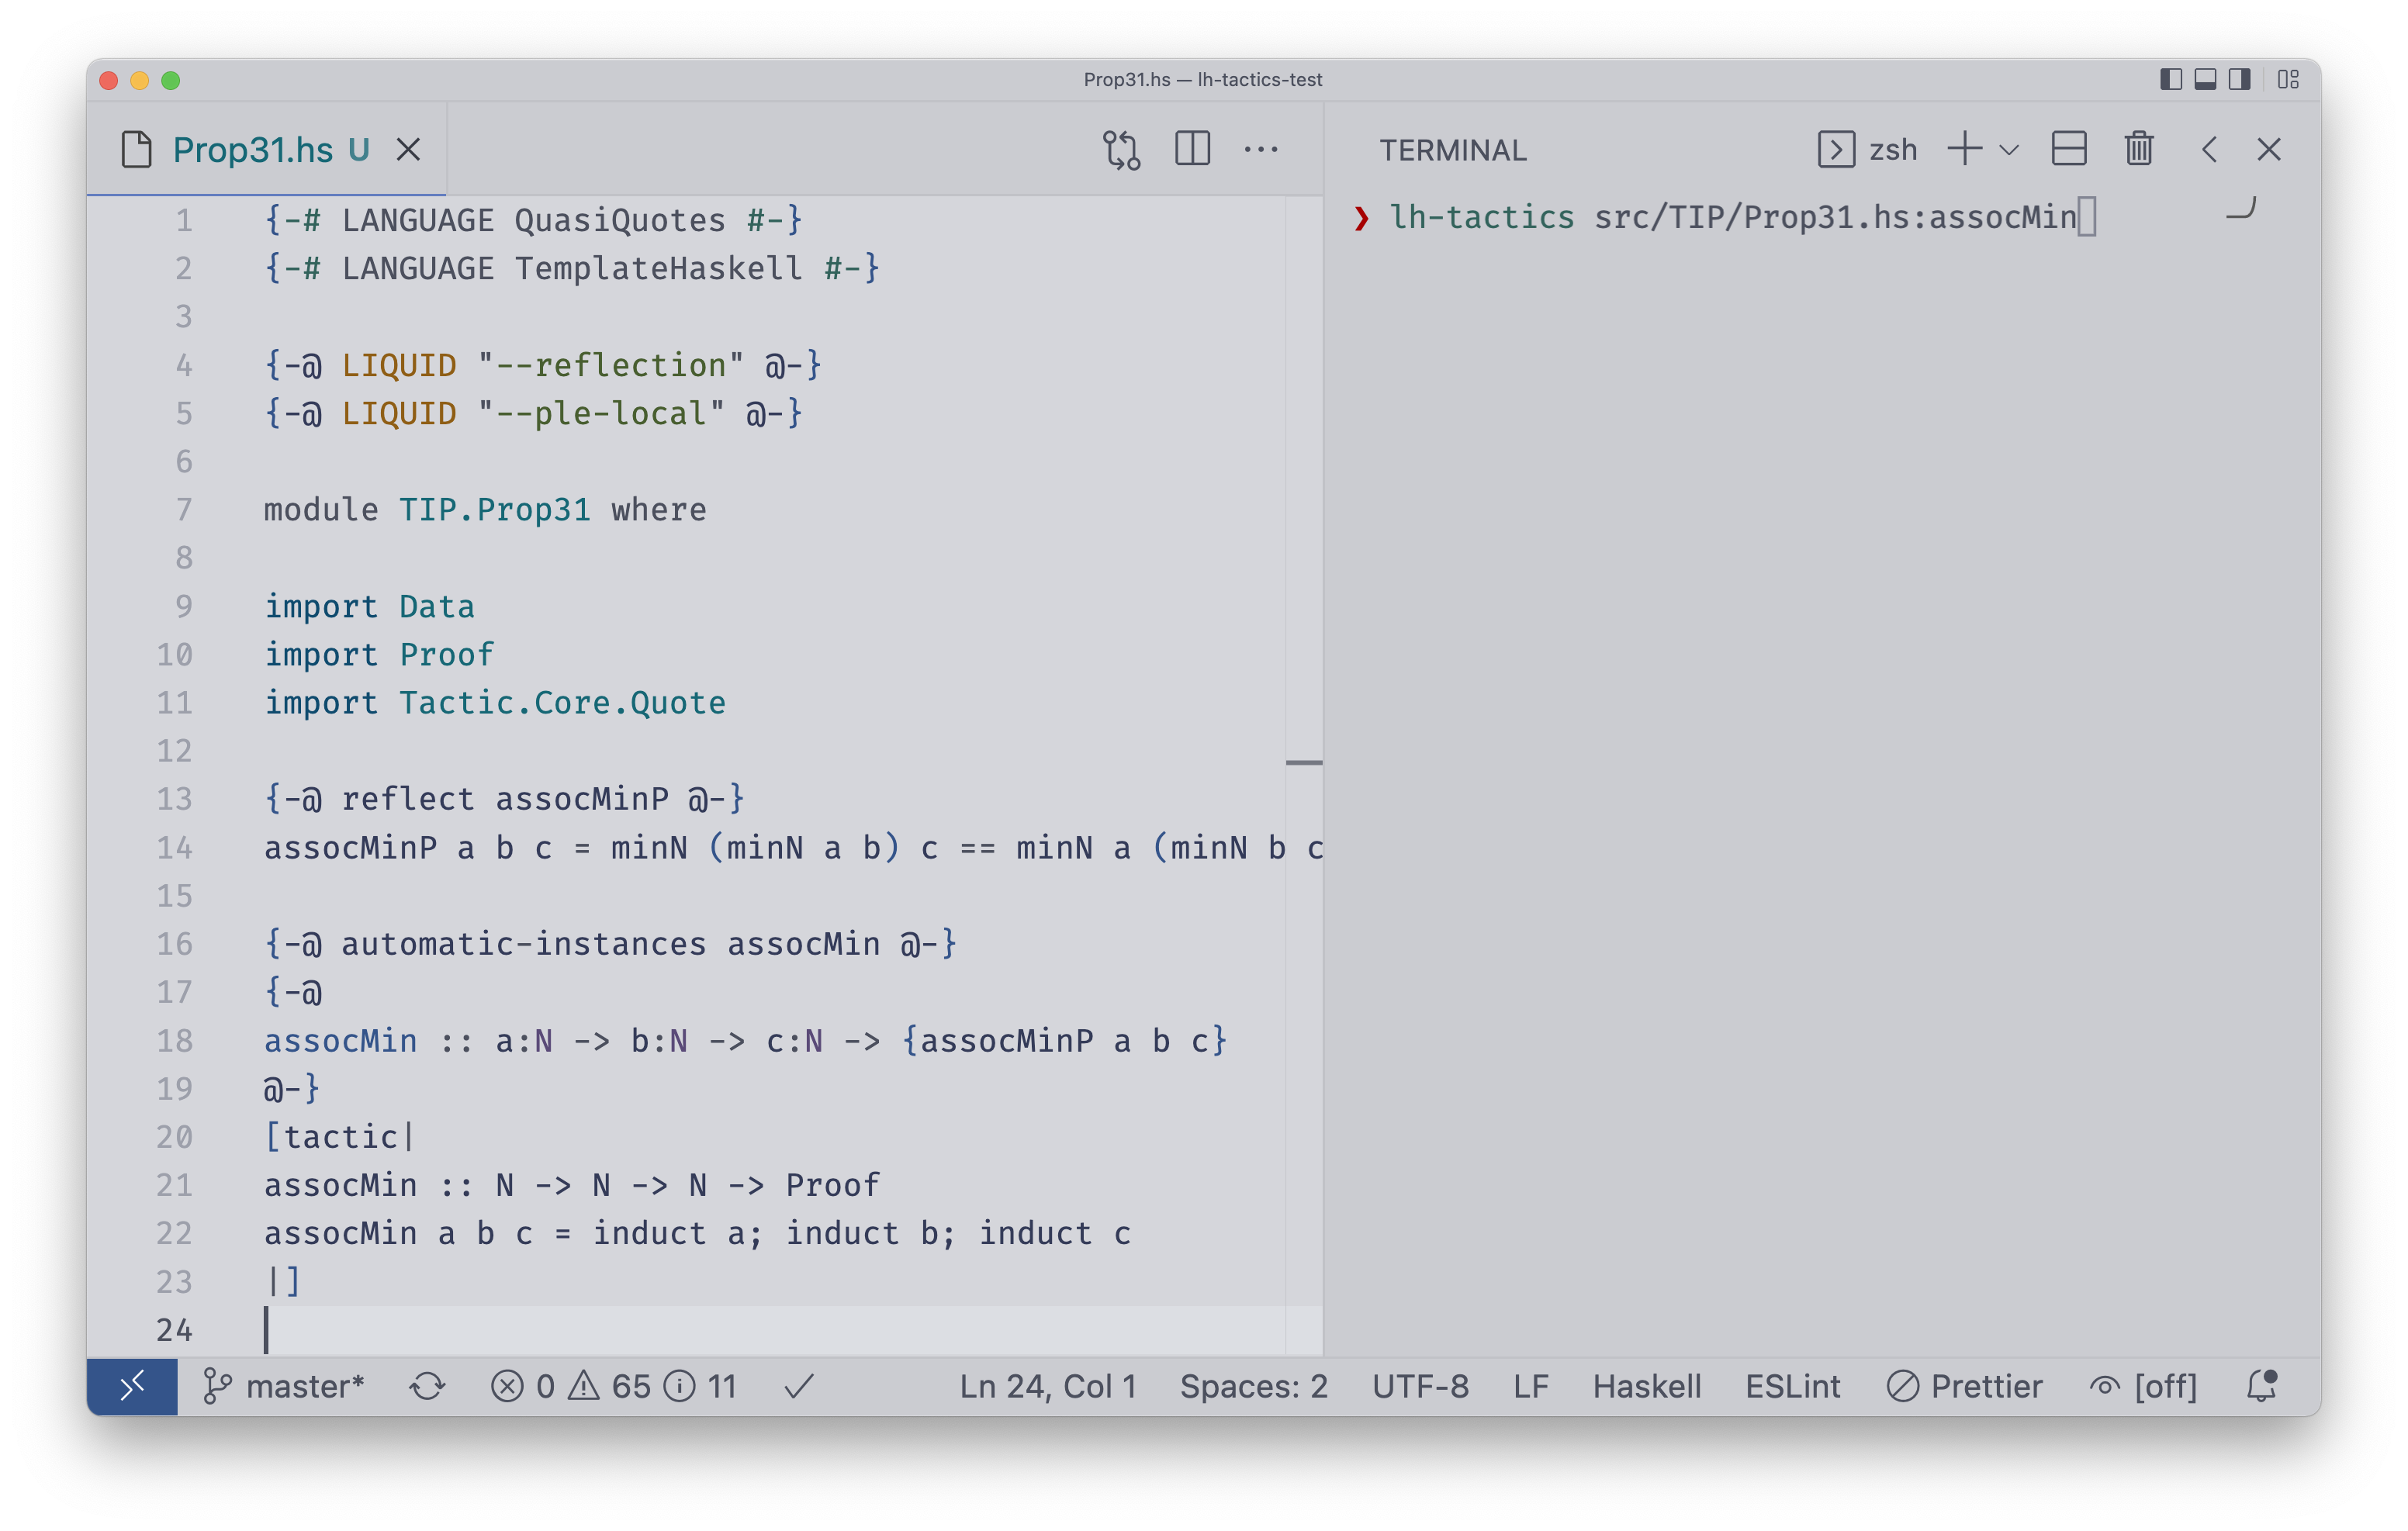
\includegraphics[width=\textwidth]{example-screenshots/run.png}
    \end{minipage}
  \end{subfigure}
  \begin{subfigure}[t][][t]{1\textwidth}
    % \centering
    \begin{minipage}[c]{0.5\textwidth}
      \caption{The user waits for the \LC{lh-tactics} tool to complete. During
      this time, the tool will overwrite the input file on each pruning attempt.}
    \end{minipage}
    \hfill
    \begin{minipage}[c]{0.49\textwidth}
      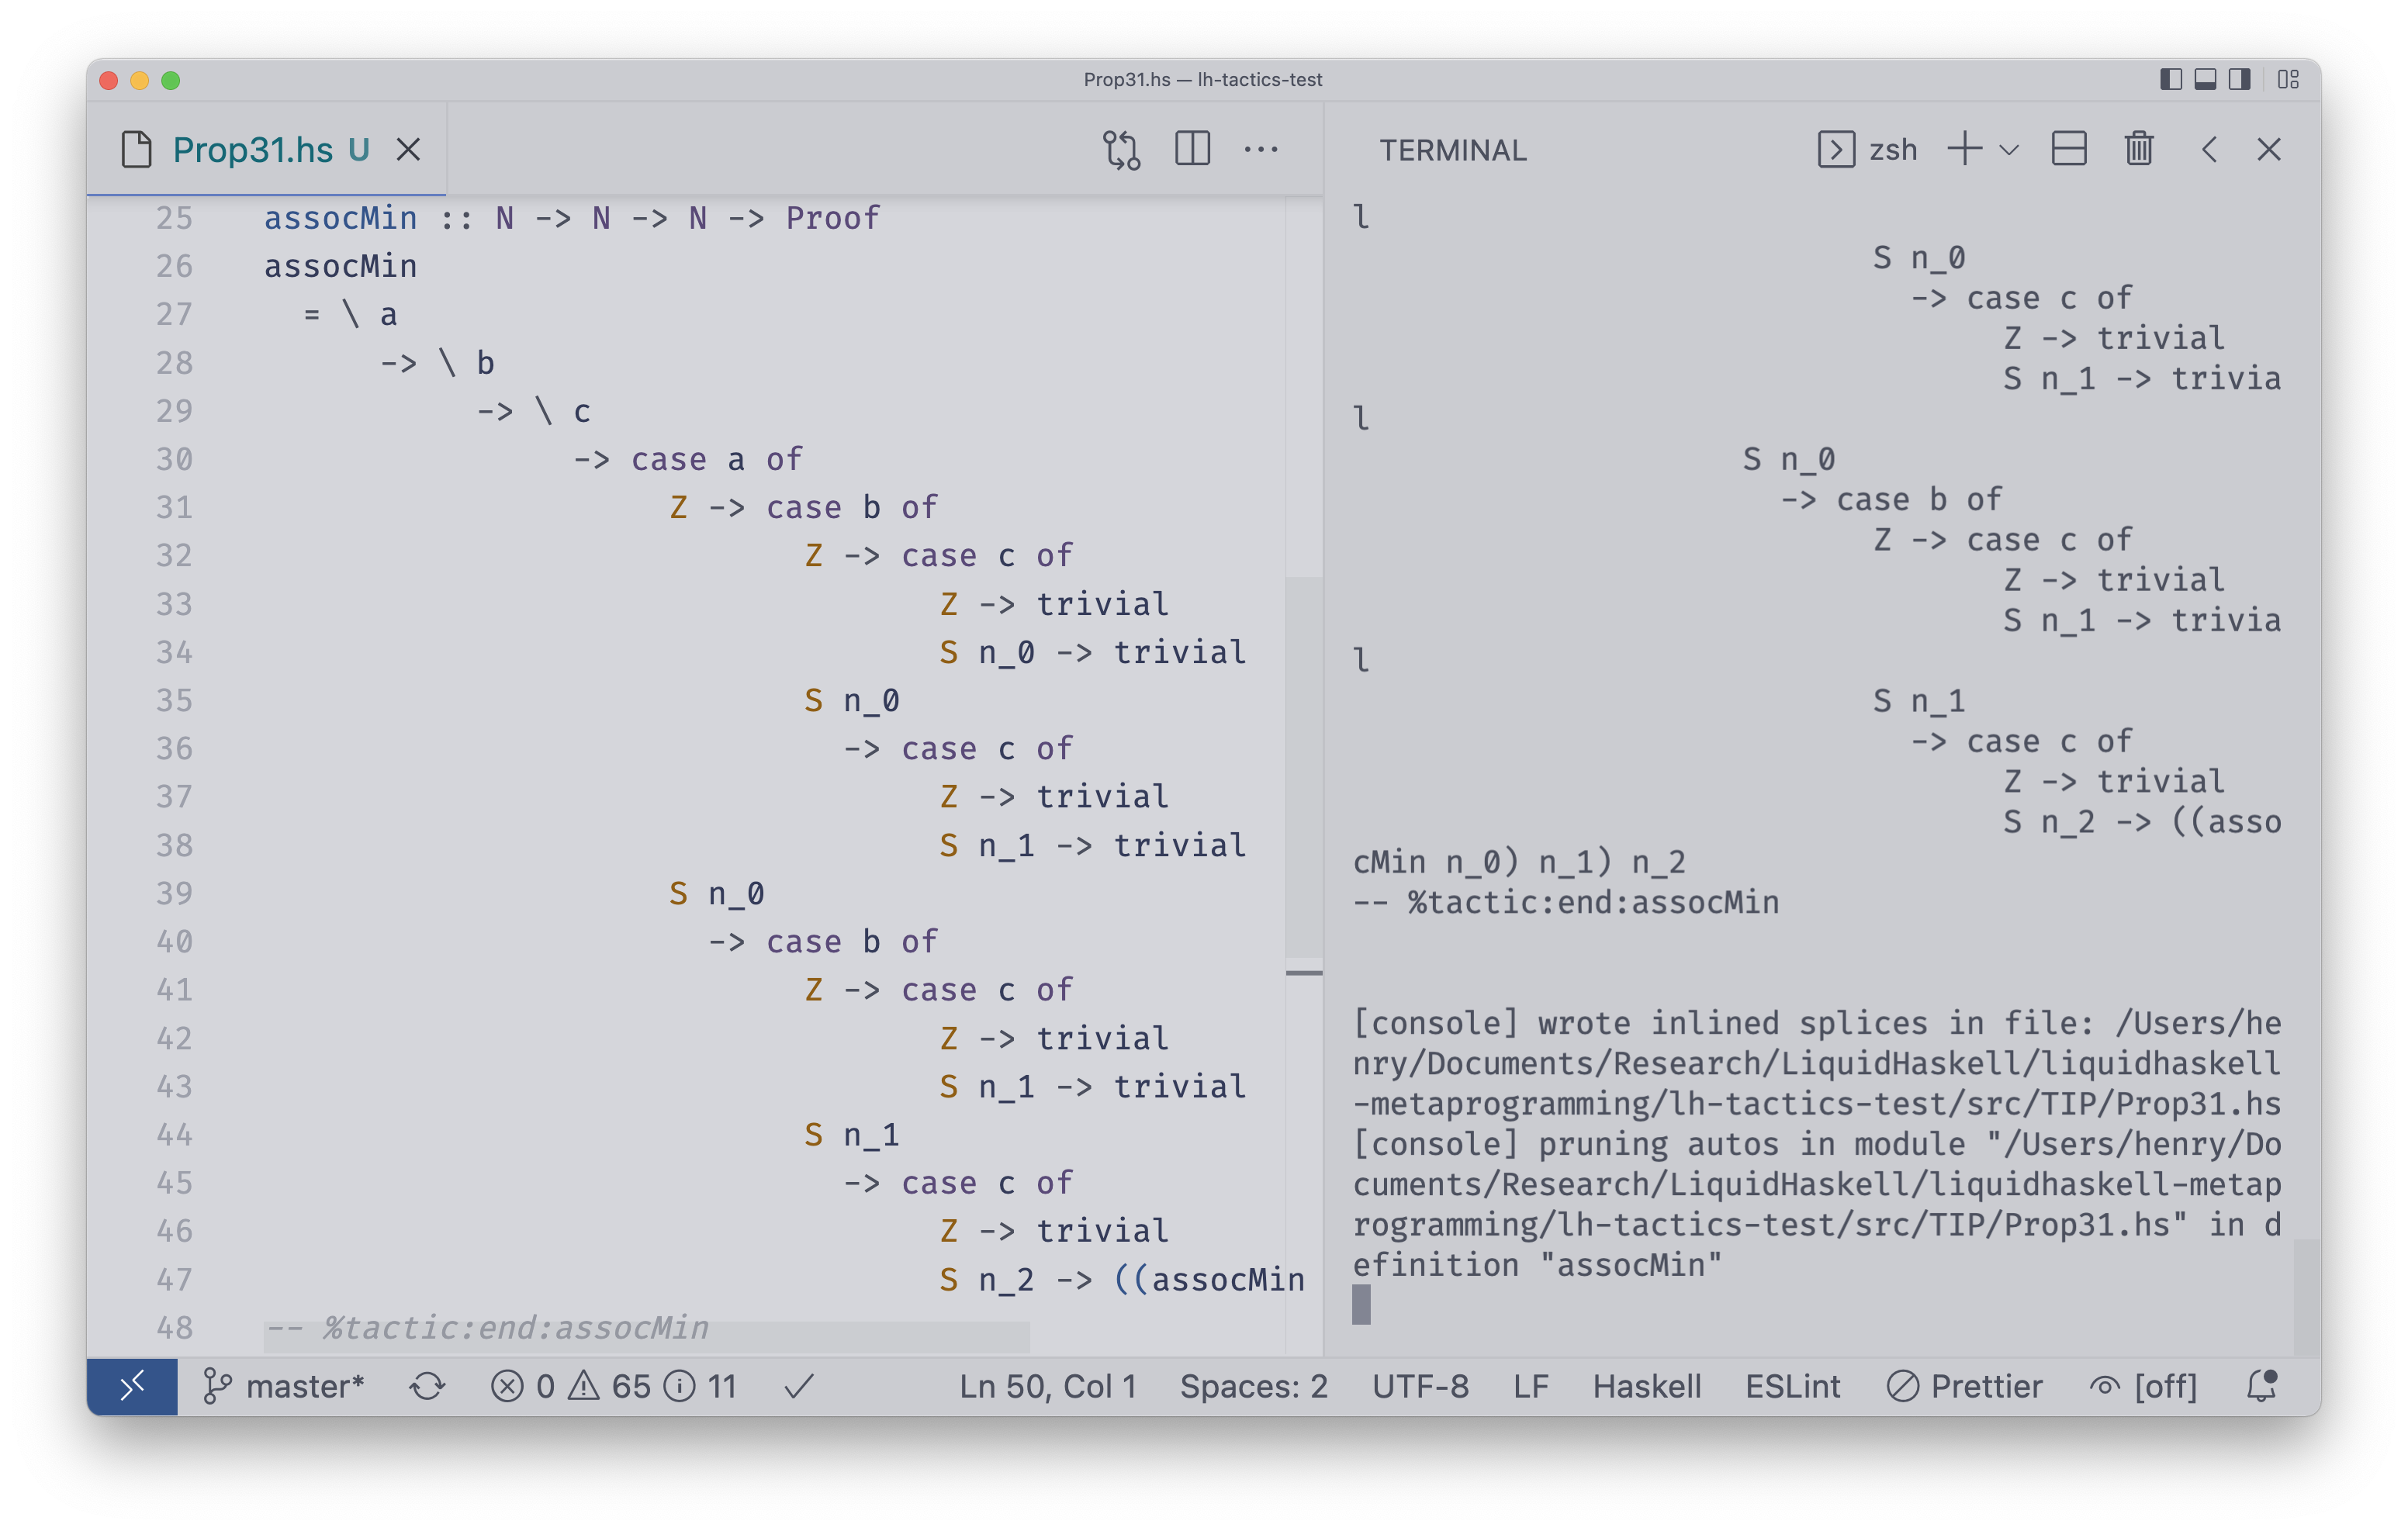
\includegraphics[width=\textwidth]{example-screenshots/pruning.png}
    \end{minipage}
  \end{subfigure}
  \begin{subfigure}[t][][t]{1\textwidth}
    % \centering
    \begin{minipage}[c]{0.5\textwidth}
      \caption{Once pruning has completed, the final proof term is presented and
      the original proof macros that generated it are left in a comment 
      immediately above.}    \end{minipage}
    \hfill
    \begin{minipage}[c]{0.49\textwidth}
      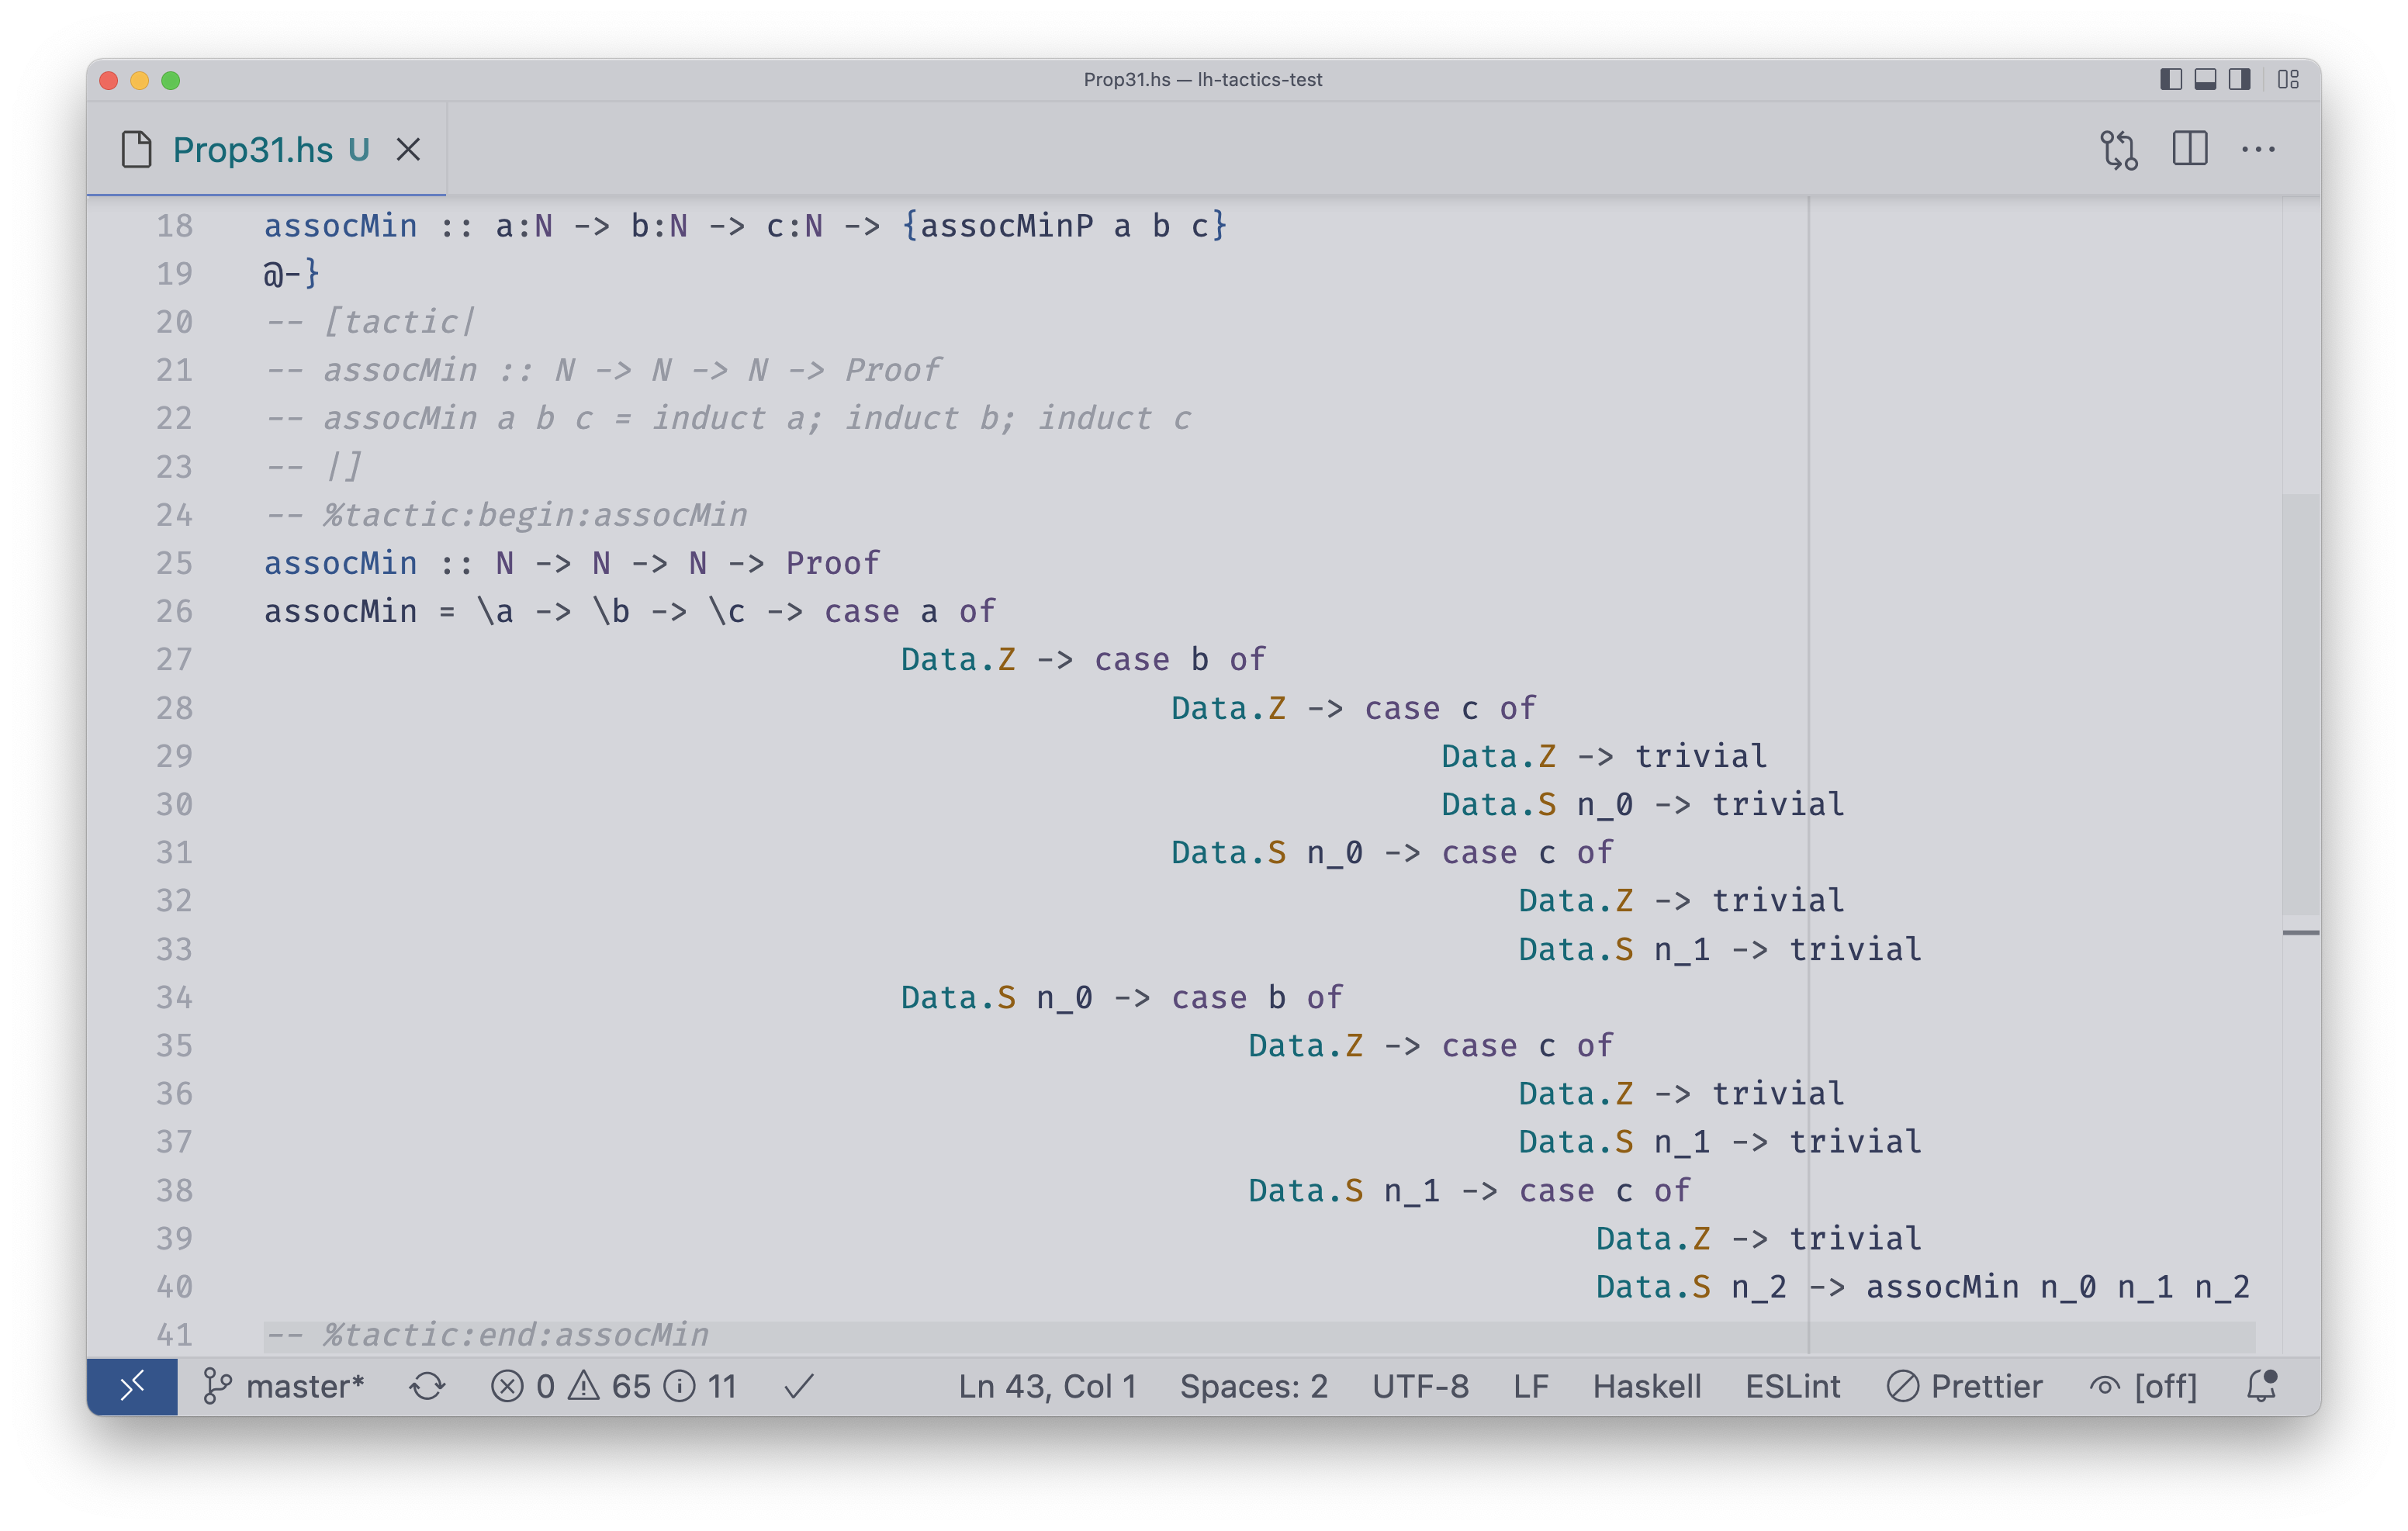
\includegraphics[width=\textwidth]{example-screenshots/done.png}
    \end{minipage}
  \end{subfigure}
  % &
  % \begin{subfigure}[t][][t]{1\textwidth}
  %   \centering
  %   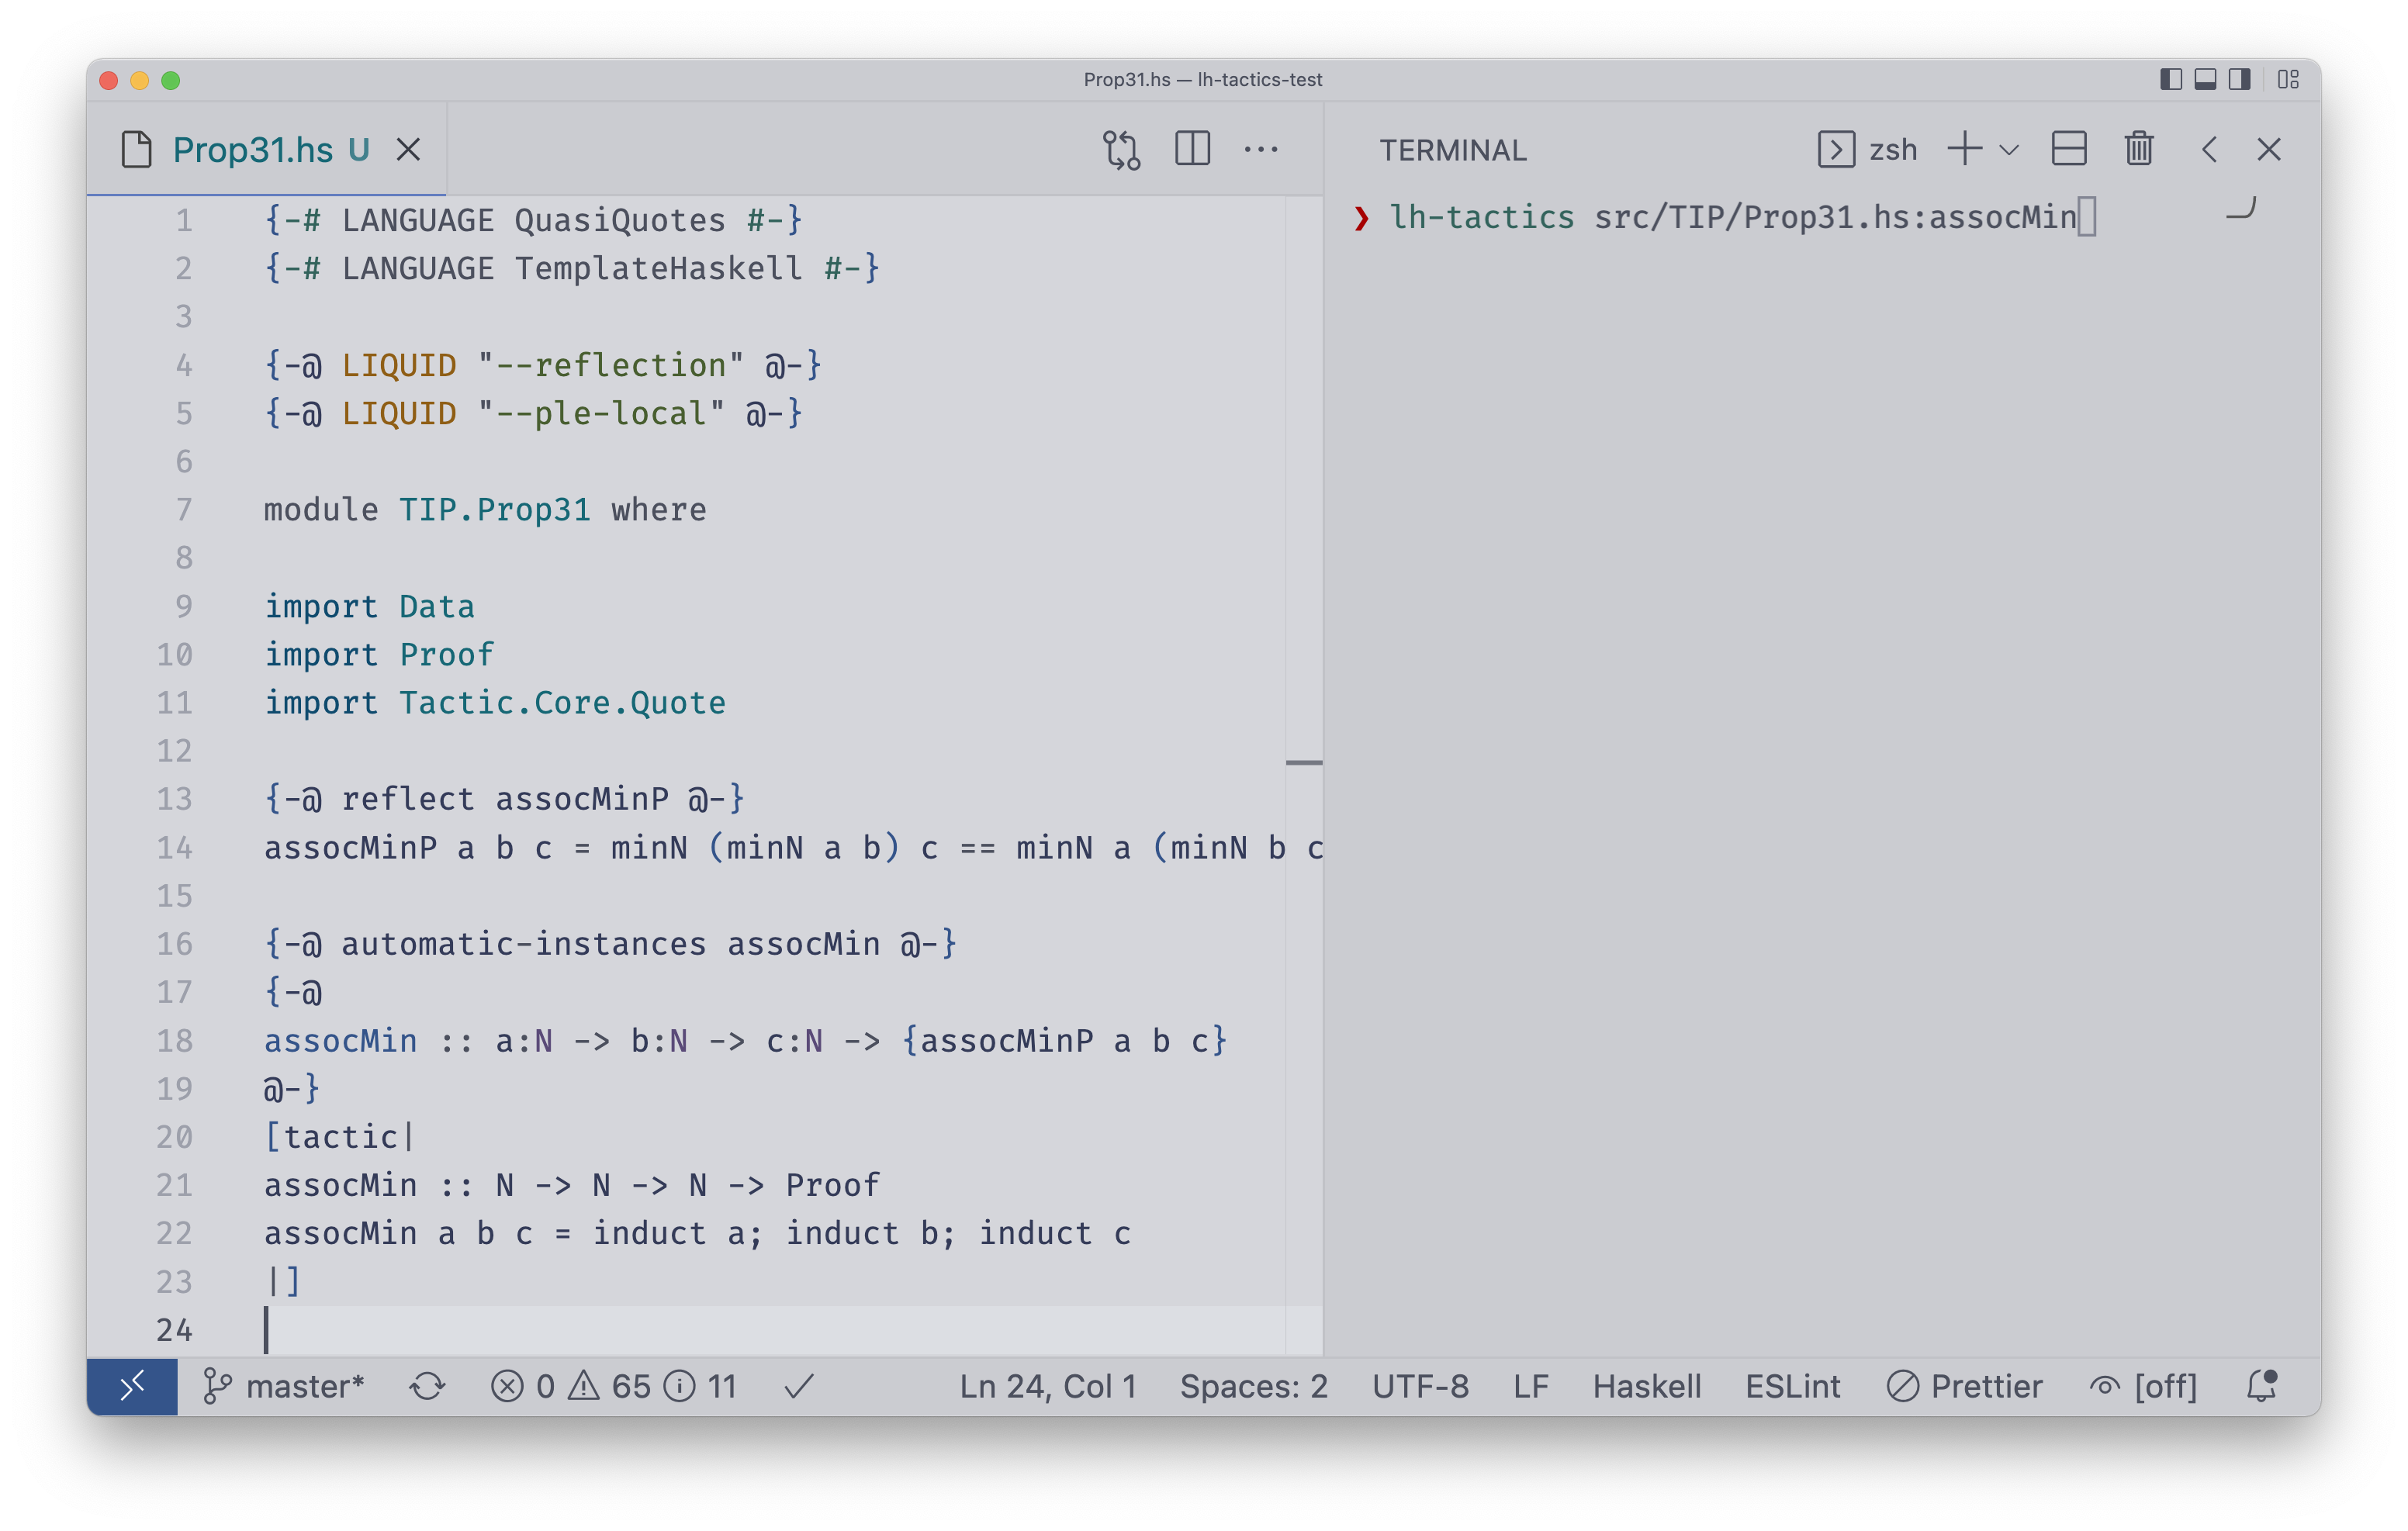
\includegraphics[width=\textwidth]{example-screenshots/run.png}
  %   \caption{The user runs the \LC{lh-tactics} command line tool on the input
  %   file, which exists inside of a \textit{stack} project that is configured to
  %   use the LiquidHaskell as a plugin.}
  % \end{subfigure}
  % % \\
  % \begin{subfigure}[t][][t]{1\textwidth}
  %   \centering
  %   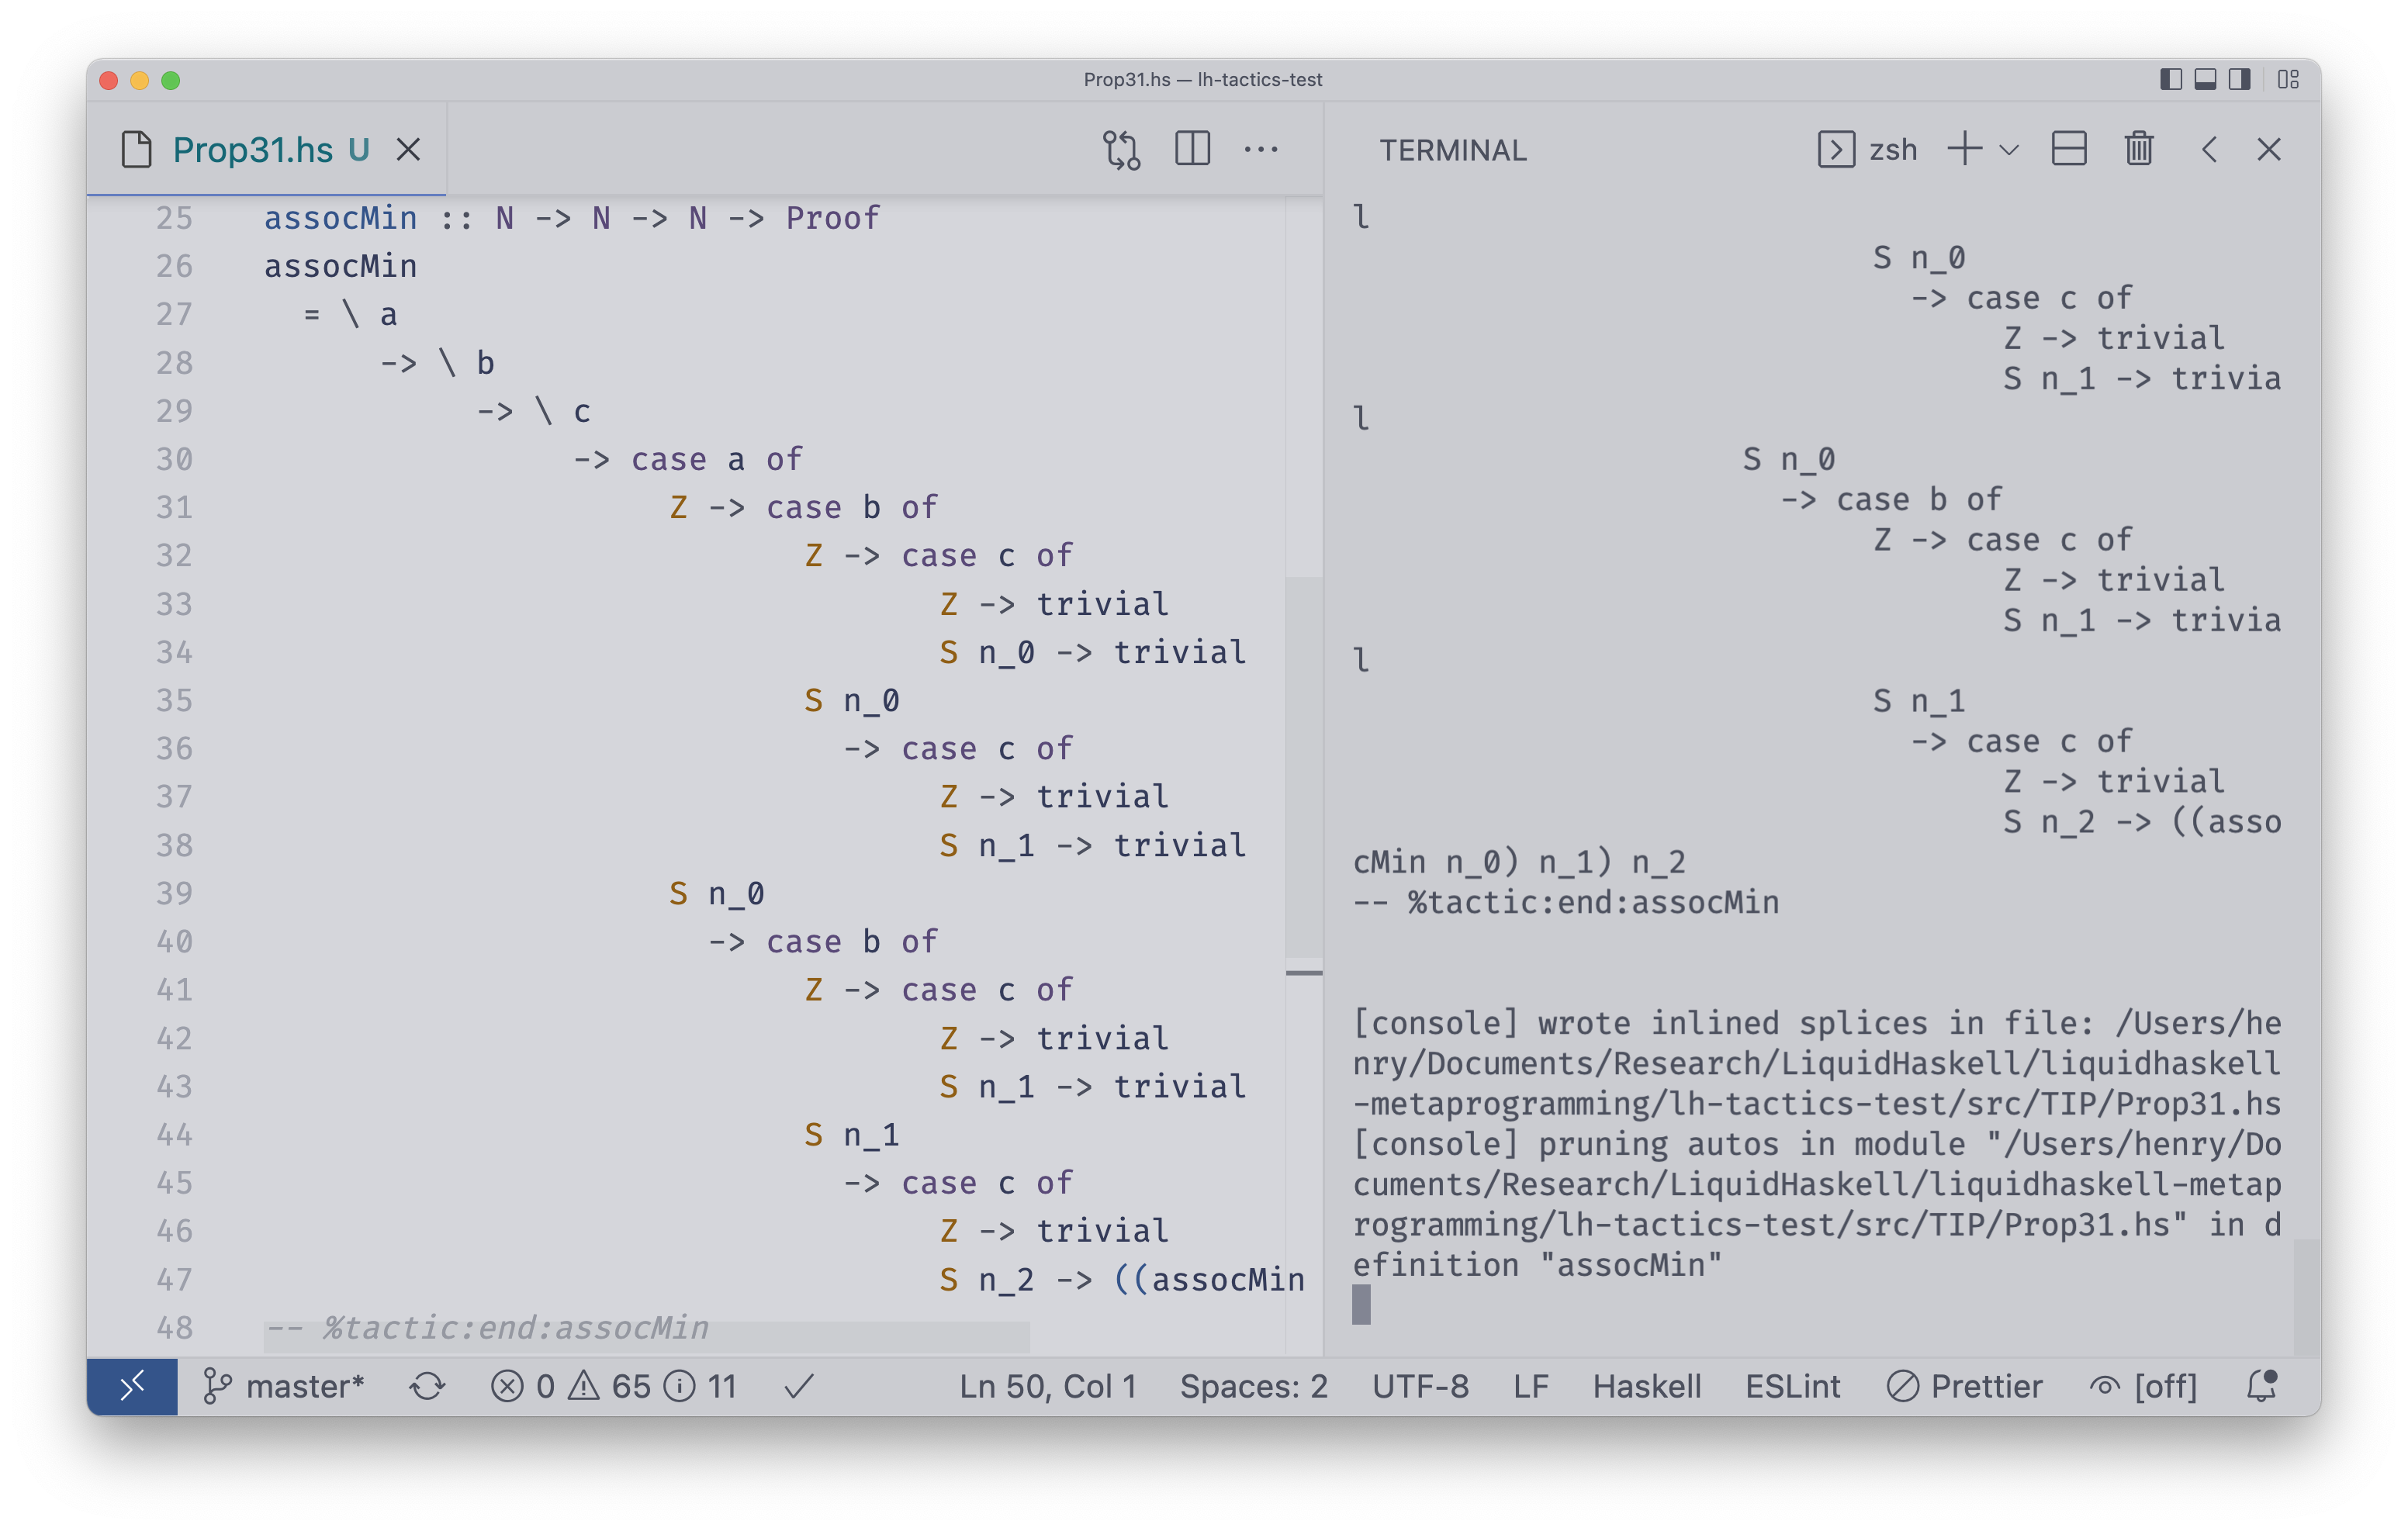
\includegraphics[width=\textwidth]{example-screenshots/pruning.png}
  %   \caption{The user waits for the \LC{lh-tactics} tool to complete. During
  %   this time, the tool will overwrite the input file on each pruning attempt.}
  % \end{subfigure}
  % % &
  % \begin{subfigure}[t][][t]{1\textwidth}
  %   \centering
  %   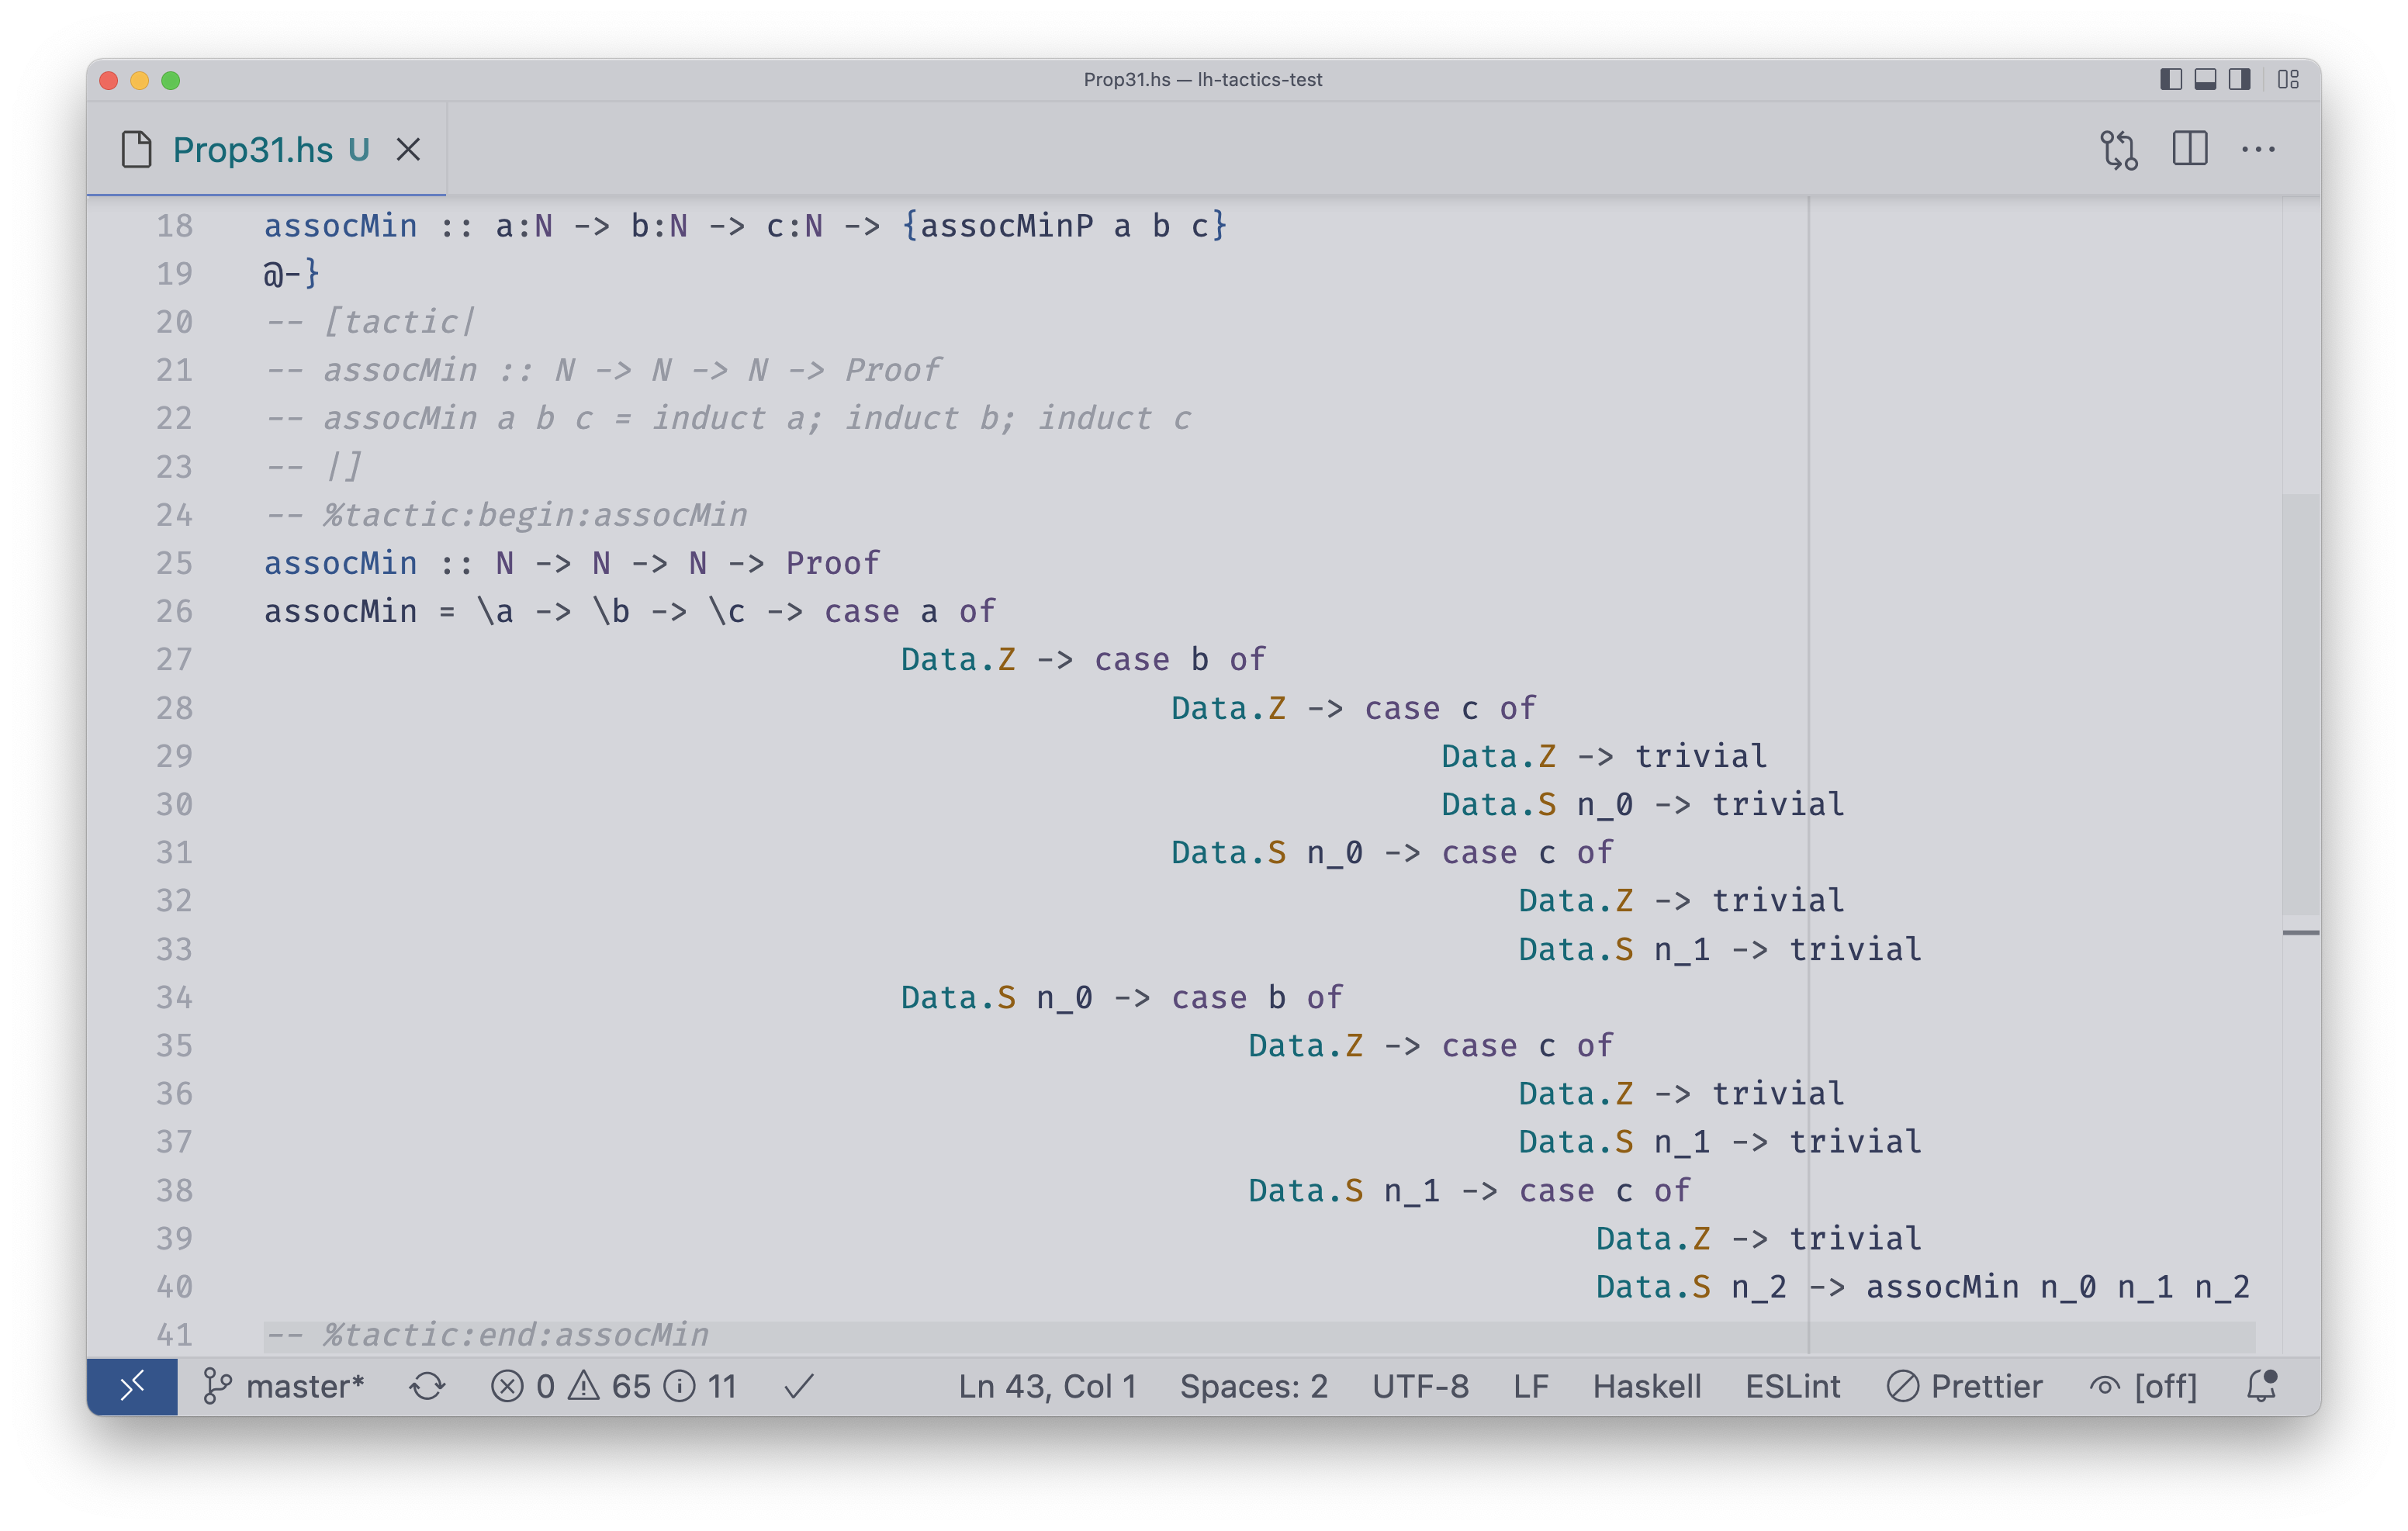
\includegraphics[width=\textwidth]{example-screenshots/done.png}
  %   \caption{Once pruning has completed, the final proof term is presented and
  %   the original proof macros that generated it are left in a comment 
  %   immediately above.}
  % \end{subfigure}

  % \begin{tabular}{cc}
  %   \begin{subfigure}[t][][t]{0.49\textwidth}
  %     \centering
  %     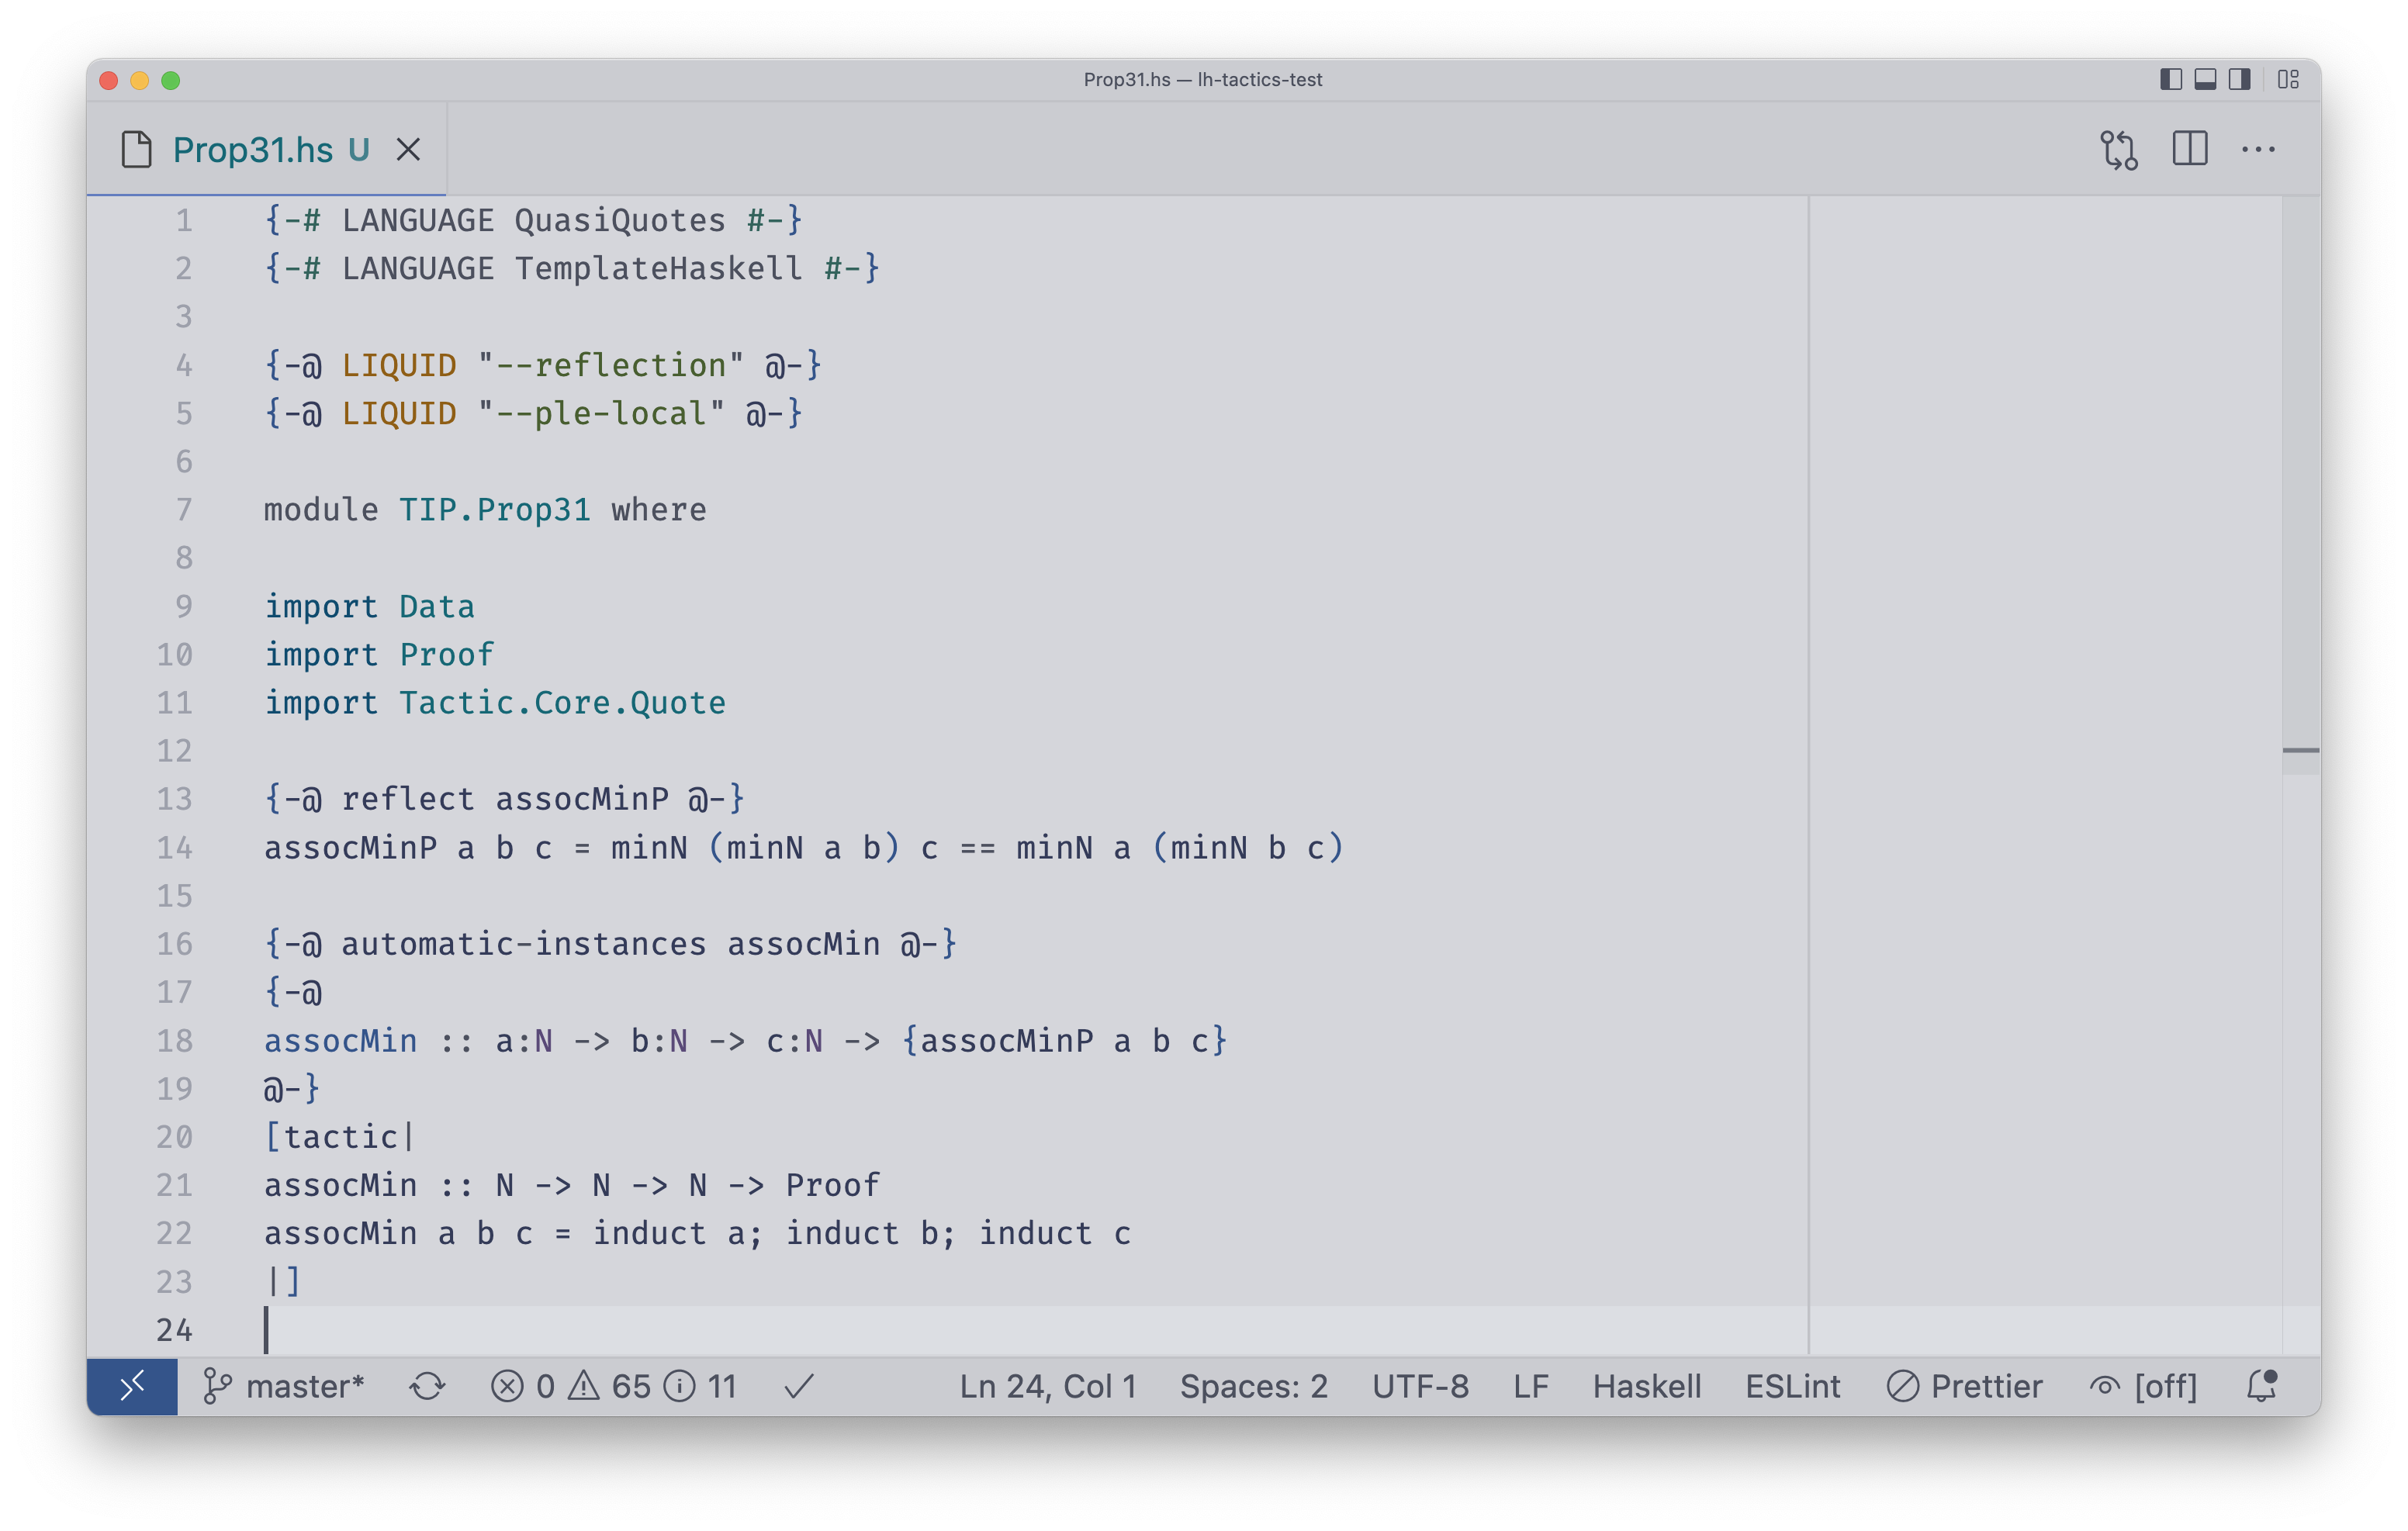
\includegraphics[width=\textwidth]{example-screenshots/macros.png}
  %     \caption{The user writes the proof macros.}
  %   \end{subfigure}
  %   &
  %   \begin{subfigure}[t][][t]{0.49\textwidth}
  %     \centering
  %     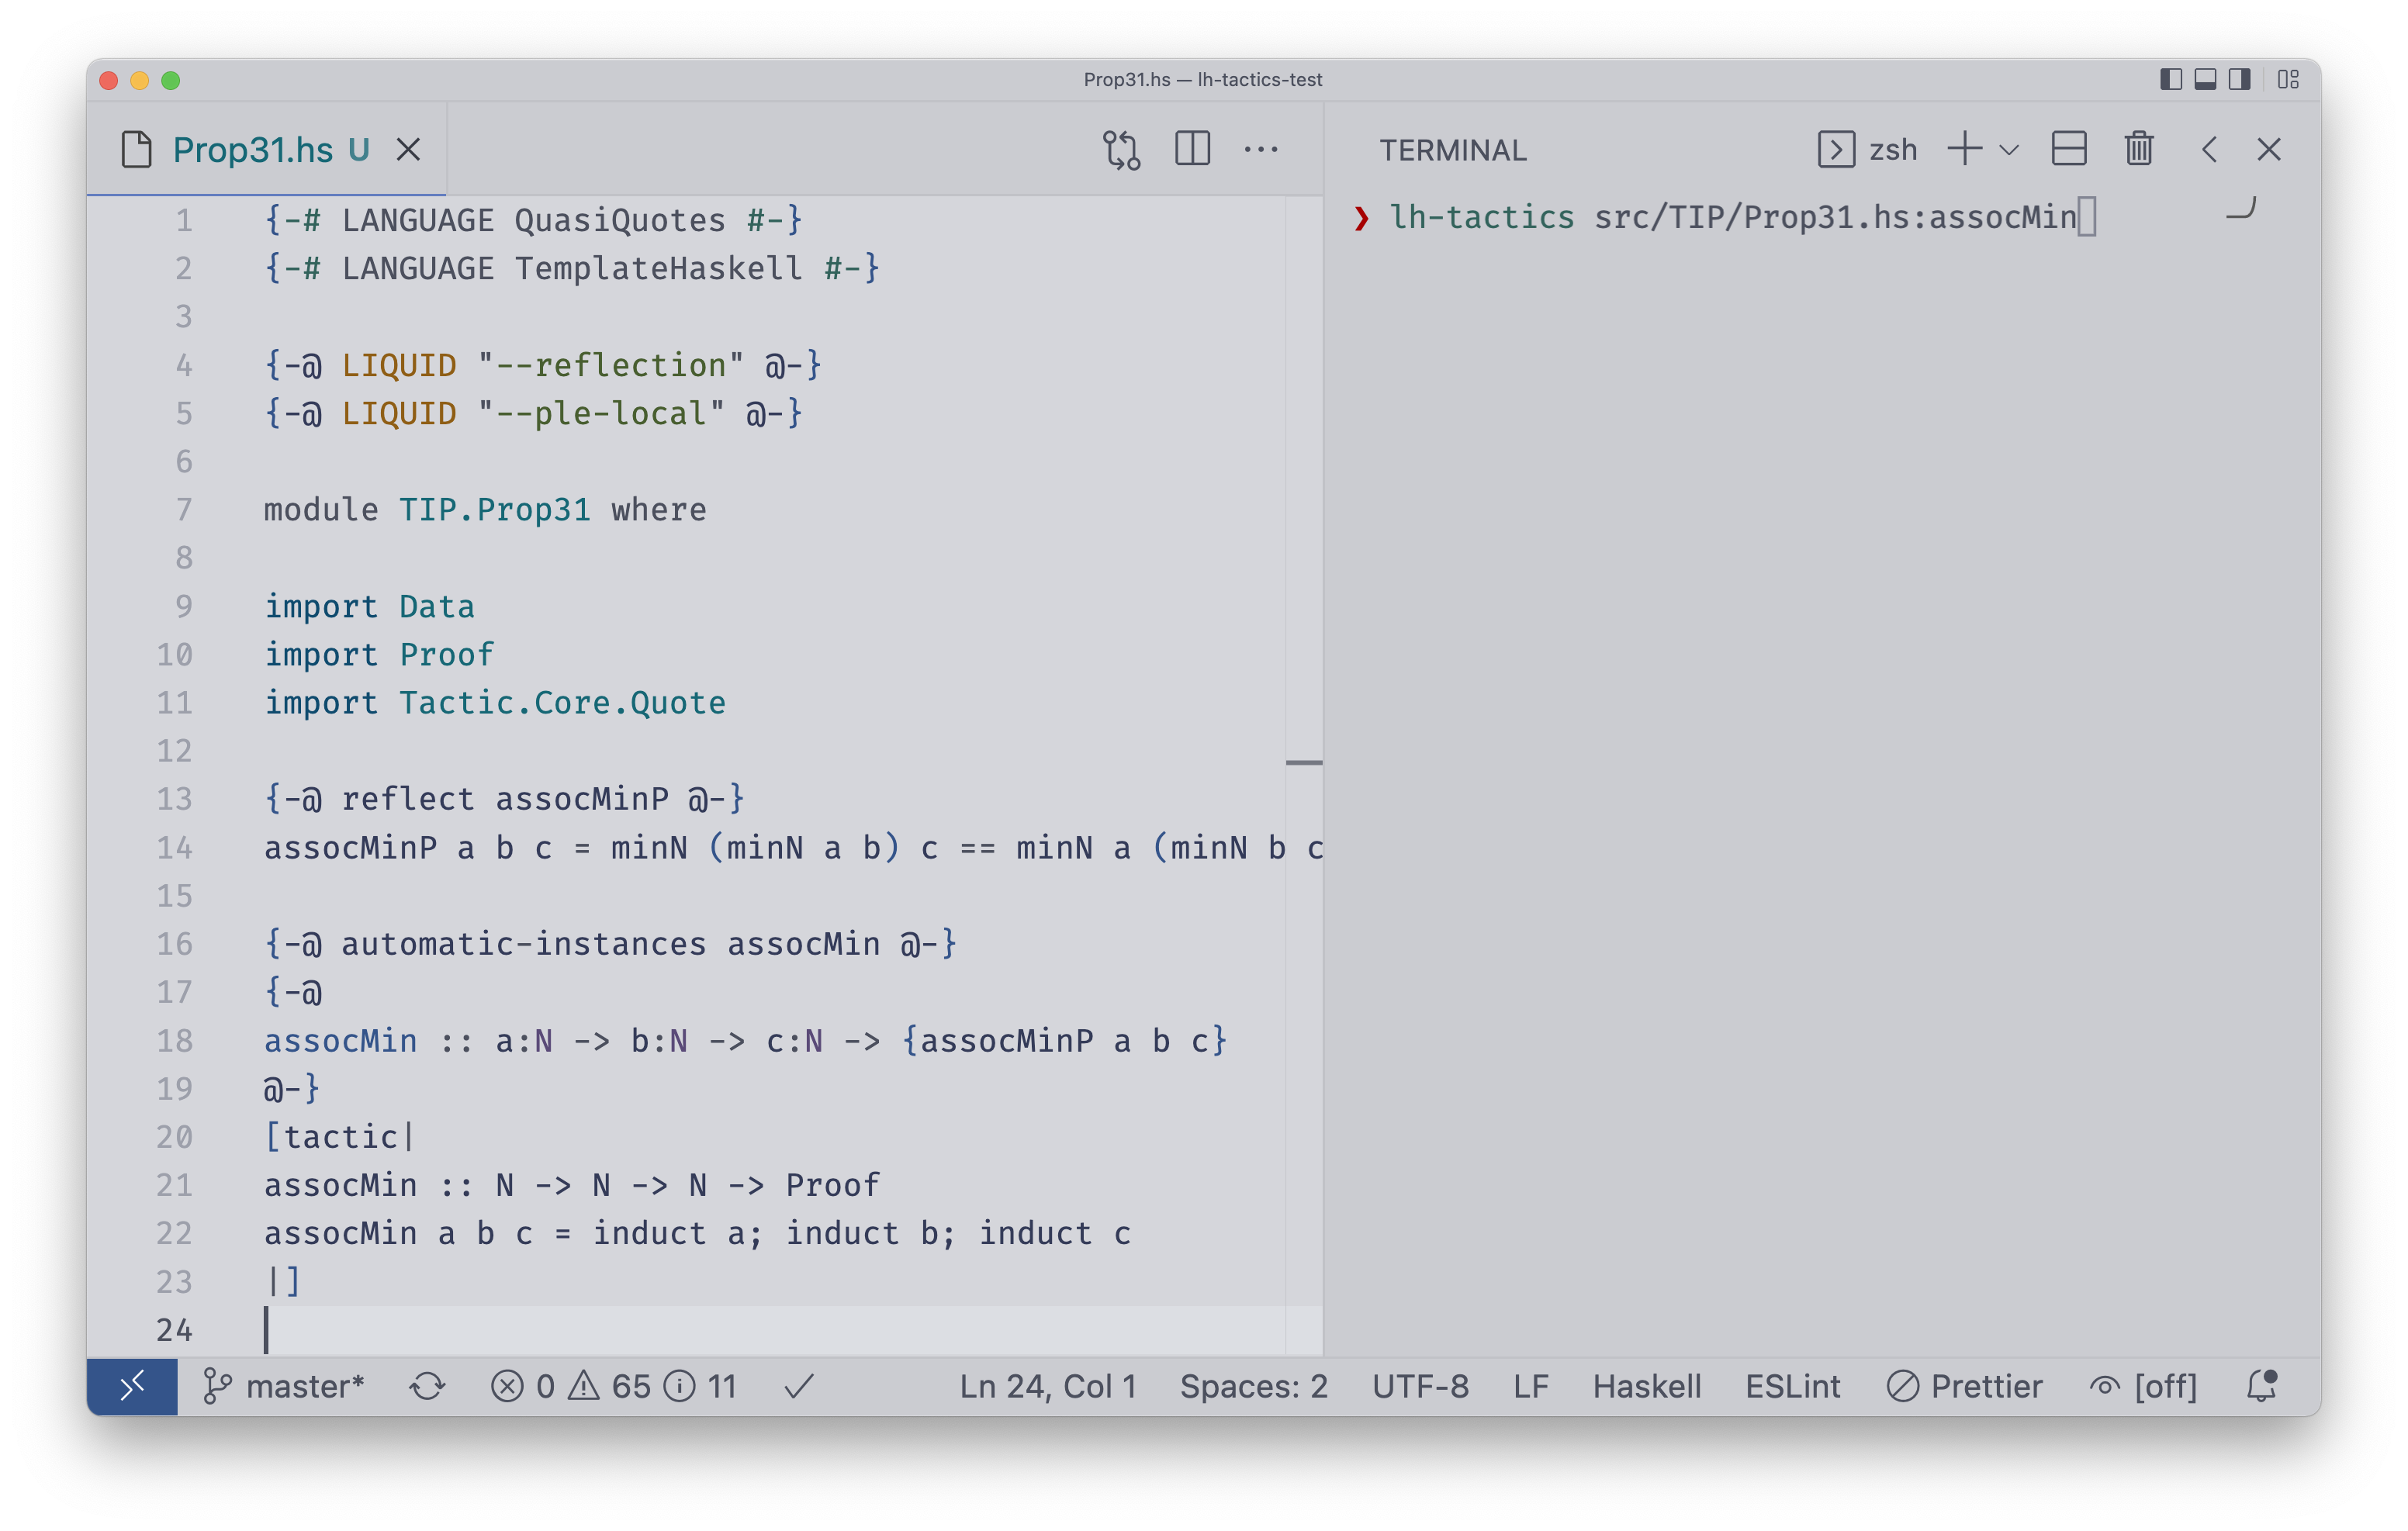
\includegraphics[width=\textwidth]{example-screenshots/run.png}
  %     \caption{The user runs the \LC{lh-tactics} command line tool on the input
  %     file, which exists inside of a \textit{stack} project that is configured to
  %     use the LiquidHaskell as a plugin.}
  %   \end{subfigure}
  %   \\
  %   \begin{subfigure}[t][][t]{0.49\textwidth}
  %     \centering
  %     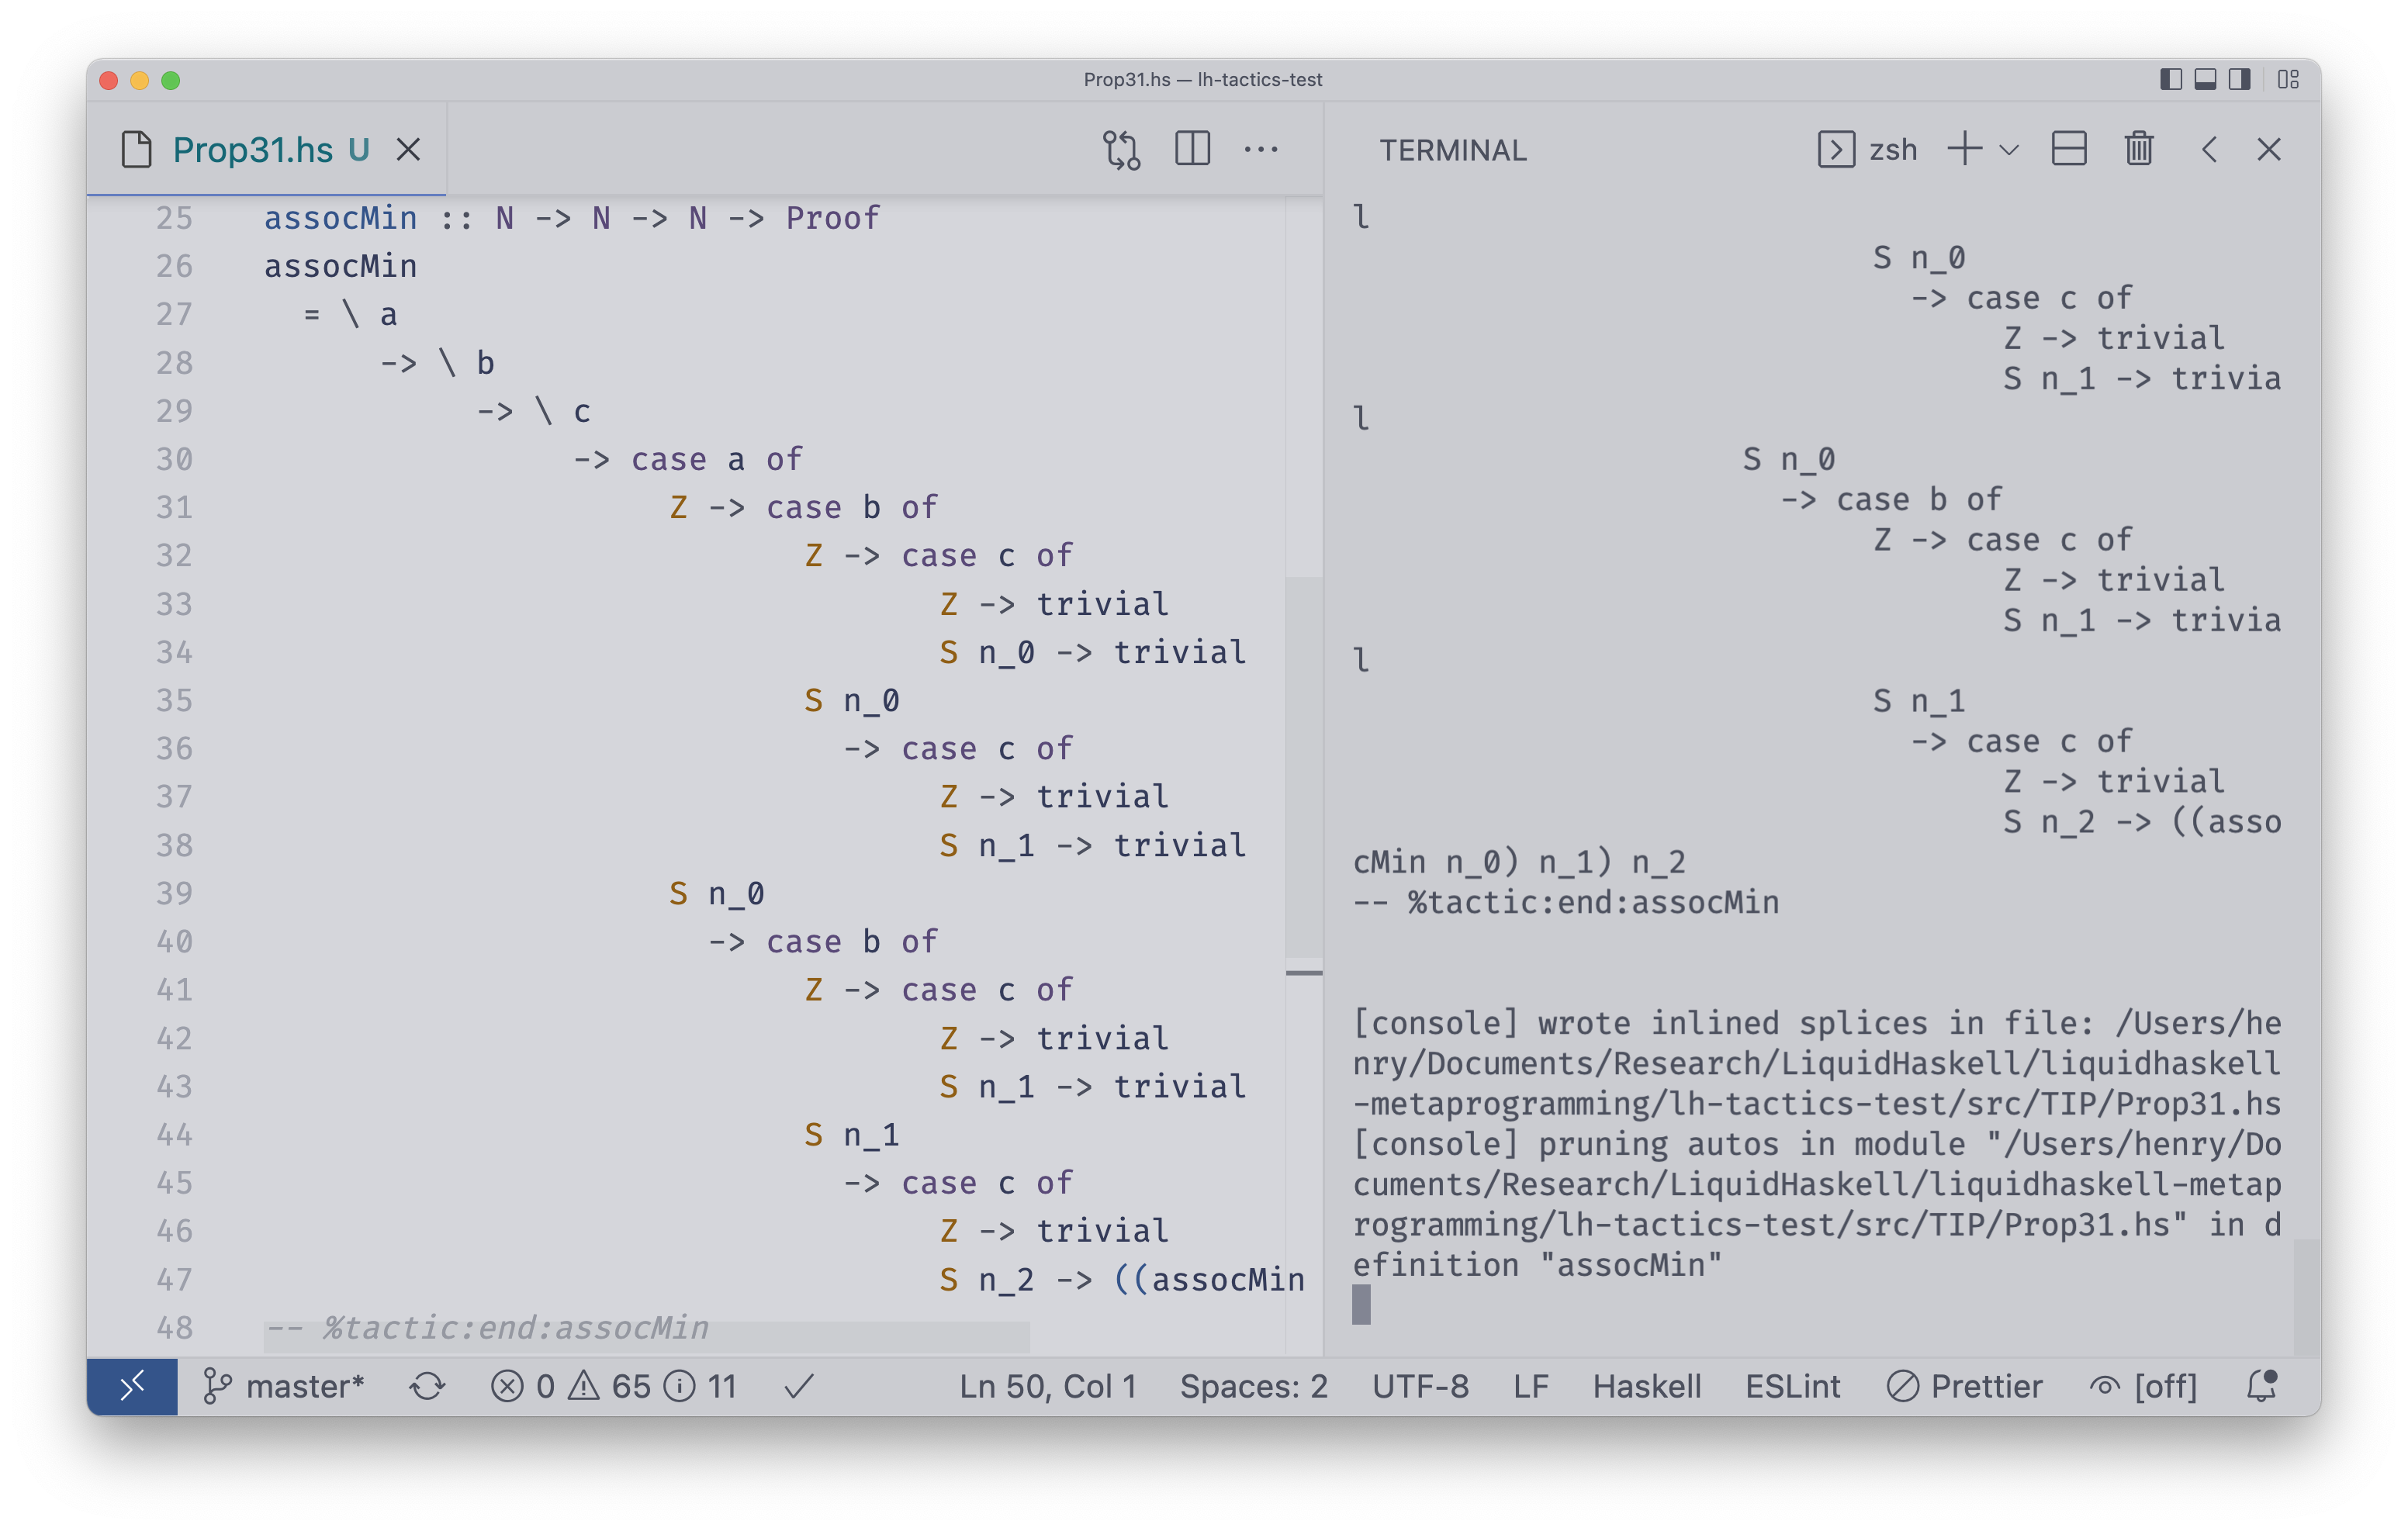
\includegraphics[width=\textwidth]{example-screenshots/pruning.png}
  %     \caption{The user waits for the \LC{lh-tactics} tool to complete. During
  %     this time, the tool will overwrite the input file on each pruning attempt.}
  %   \end{subfigure}
  %   &
  %   \begin{subfigure}[t][][t]{0.49\textwidth}
  %     \centering
  %     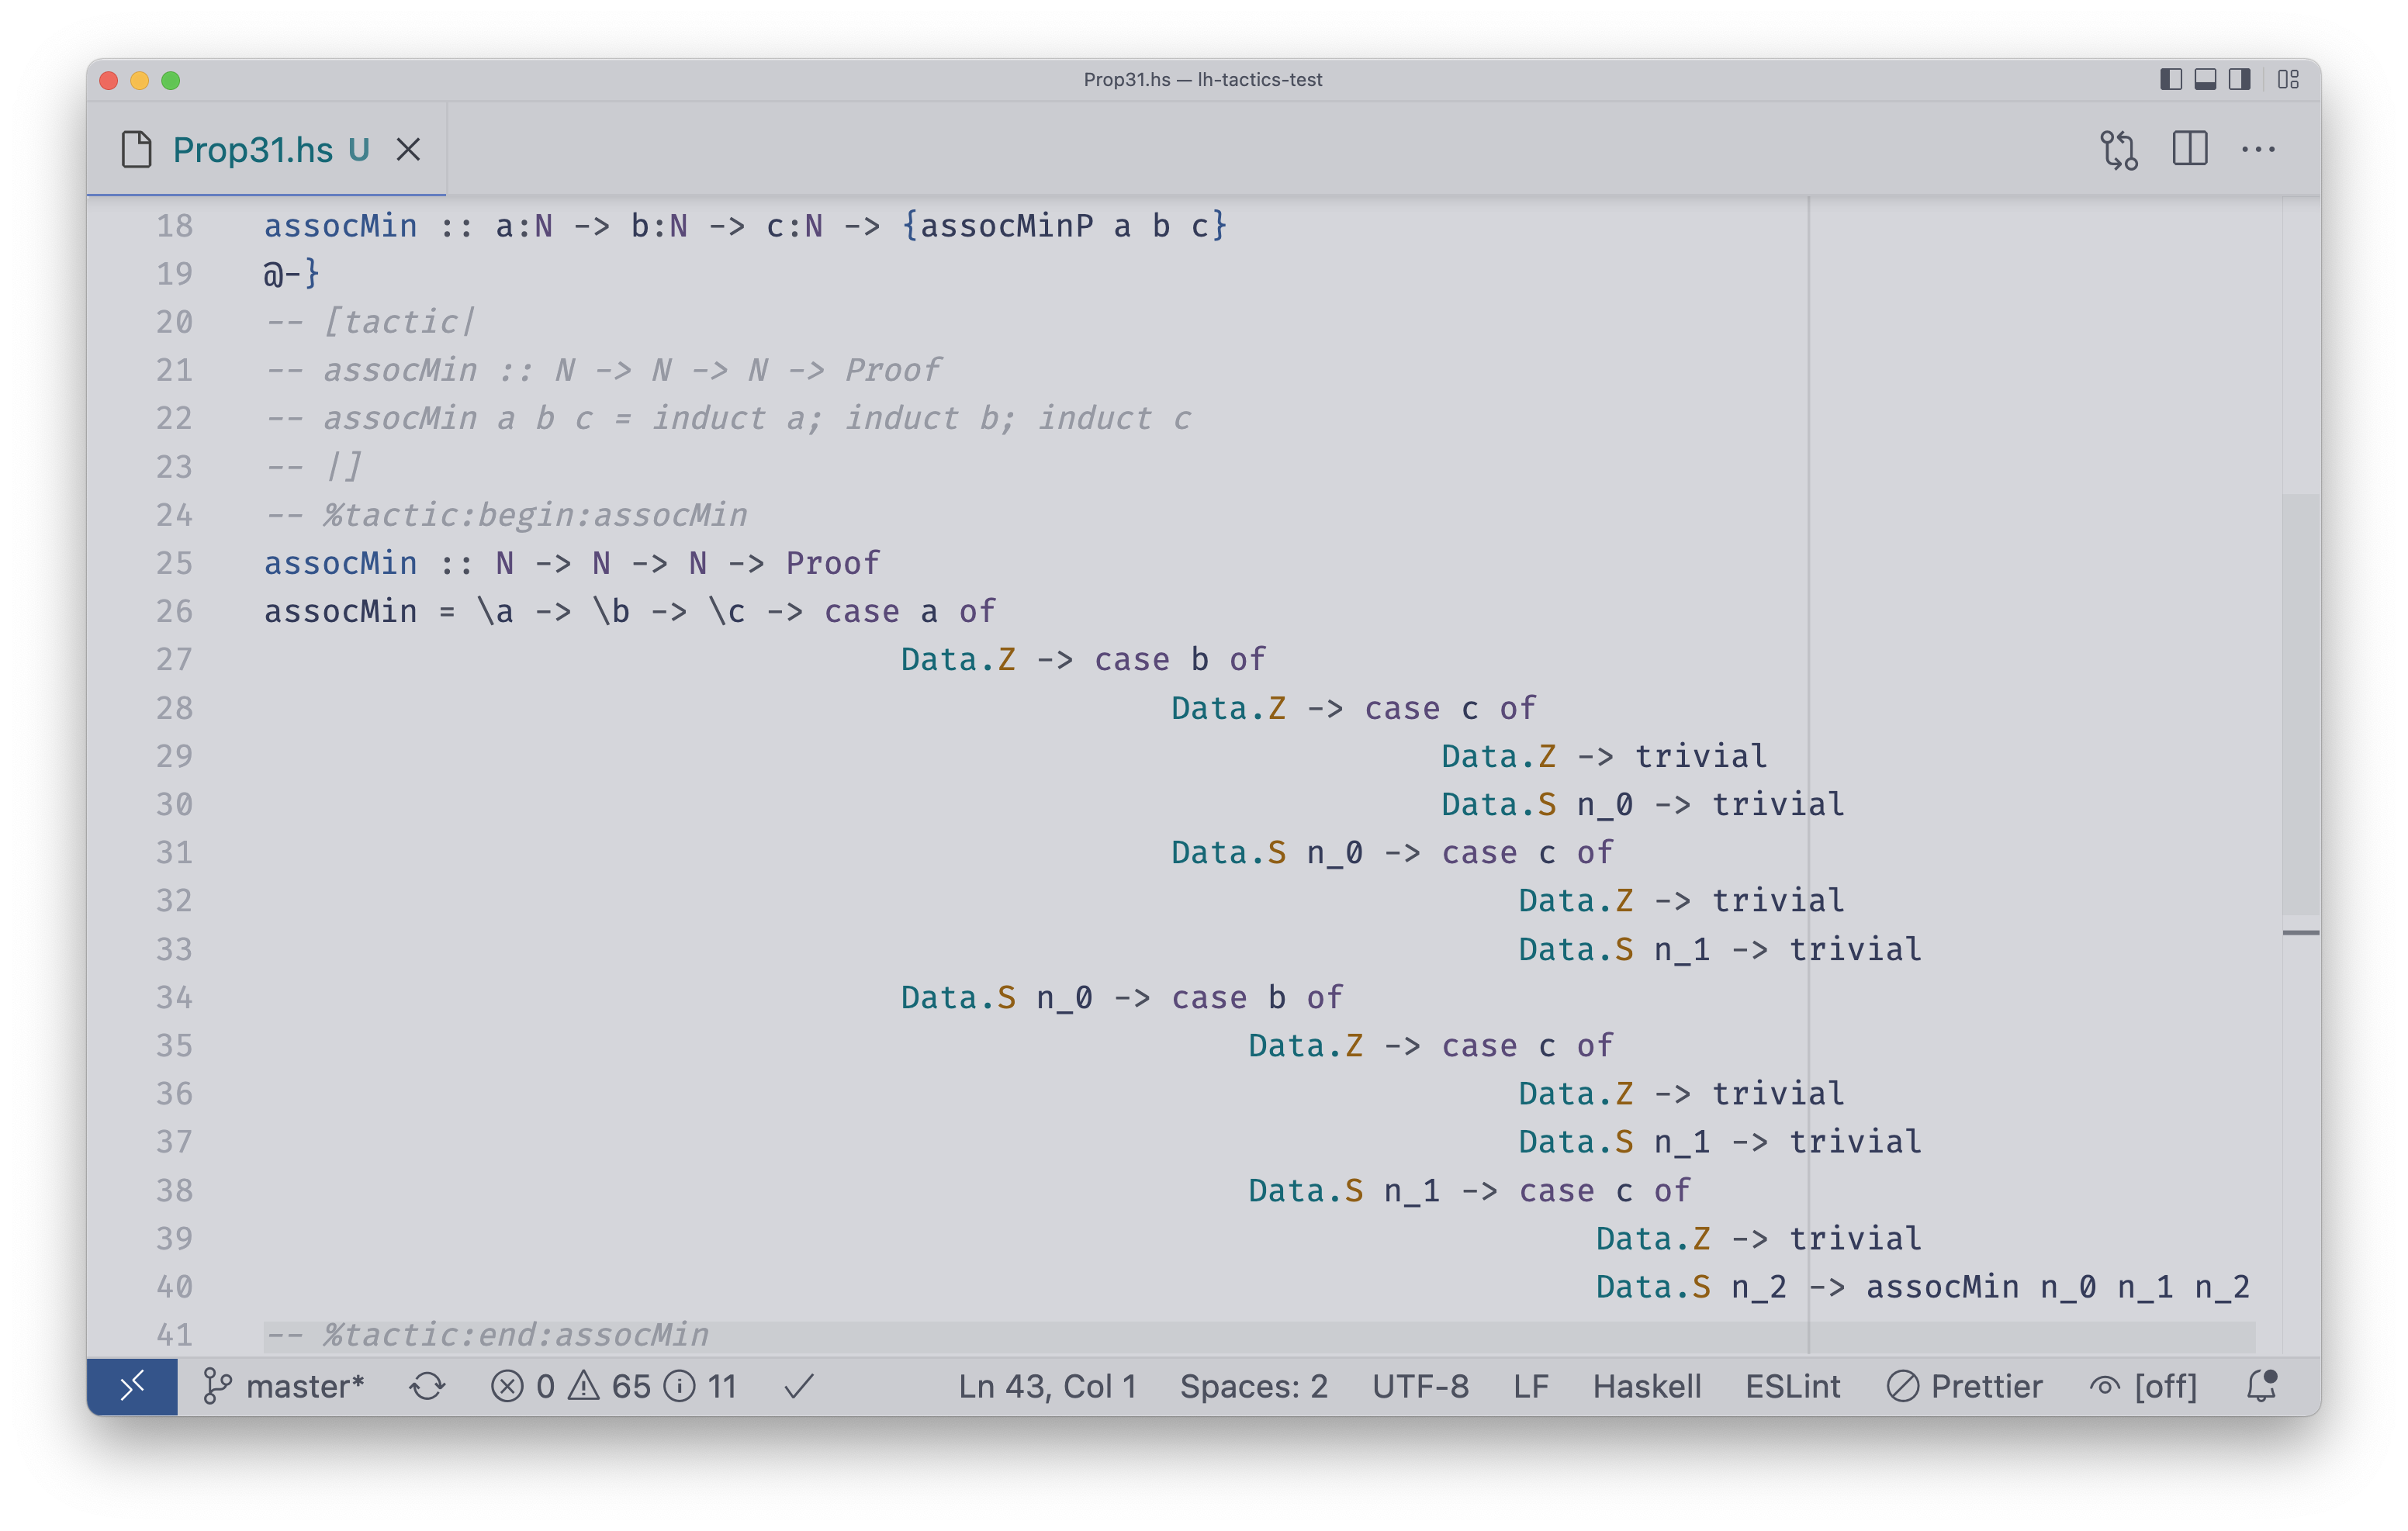
\includegraphics[width=\textwidth]{example-screenshots/done.png}
  %     \caption{Once pruning has completed, the final proof term is presented and
  %     the original proof macros that generated it are left in a comment 
  %     immediately above.}
  %   \end{subfigure}
  % \end{tabular}
  
  % \begin{minipage}{\textwidth}
  % \end{minipage}
  \caption{Usage example of the proof macros tool.}
\end{figure*}

%  
% \todo{format data better}
% \begin{figure*}
%   \begin{tabular}{ll}
%     \hline
%     Measure label & Measure value
%     \\ \hline
%     Number of inductive proof & 
%       66
%     \\
%     Number of inductive proofs solved by simple macros &
%       45 (0.68 of inductive proofs)
%     \\
%     LOC increase after macro expansion & 
%       median: 7, mean: 15.77, std: 34.66 
%     \\ 
%     LOC increase after macro expansion and pruning & 
%       median: 2, mean: 2.61, std: 3.3
%     \\
%     Number of reasonably\footnote{\todo{Define this}} prune-able proofs &
%       73 (0.92 of proofs)
%     \\ \hline
%    \end{tabular}
%   \label{fig:evaluation}
% \end{figure*}

% \leo{Maybe some interesting examples here/outlier discussion?}
% \hen{I could include an example where the number of terms generated by auto was
% too large, so I had to manually provide lemma applications myself using the
% \macro{use} macro.
% Here's one below}
%  
% \begin{code}
%   {-@ sub_m_Sn ::  m:N -> n:N -> 
%         {subN m n == S (subN m (S n))} @-}
%  
%   {-@ sub_Sm_n_Sk :: m:N -> n:N -> k:N -> 
%         {(S m - n) - S k == (m - n) - k} @-}
%   [tactic|
%   sub_Sm_n_Sk :: N -> N -> N -> Proof
%   sub_Sm_n_Sk m n k = 
%     destruct n as [/n'];
%     use {sub_m_Sn m n'} requires [n']
%   |]
% \end{code}

% TODO OLD
% \begin{code}
%   [tactic|
%   proof :: N -> ListN -> Proof
%   proof i xs = 
%     induct i as [/i'];
%     induct xs as [/x xs'];
  
%     use {lemma4 (concatListN (reverseListN xs') (singletonListN x))} requires [xs'];
%     use {lemma1 xs'} requires [xs'];
%     use {lemma5 x xs'} requires [x, xs'];
  
%     use {lemma3'' (subN (lengthListN xs') i') (reverseListN xs') (singletonListN x)} requires [i', x, xs'];
%     use {lemma8 ((lengthListN xs')) i'} requires [i', xs'];
%     use {lemma1 xs'} requires [xs'];
%     use {proof i' xs'} requires [i', xs'];
  
%     trivial
%   |]
% \end{code}

% \todo{ideas for data to include
% \begin{itemize}
%   \item percent of inductive proofs that were proven with just ``induct x1; ...
%   induct xN''
%   \item percent of proofs that resulted in set of auto-generationed exps that
%   were too large to prune automatically
%   \item number of lines in proof macro vs number of lines in generated proof
%   term
% \end{itemize}
% }
%  
% Each of the theorems were able to be proven using the proof macro system more
% consisely than the generated proof term.
%  
% \todo{pick a few interesting examples?}

% -- prop15_lemma
%
% {-@ reflect prop15_lemma @-} prop15_lemma :: N -> N -> ListN -> Bool
% prop15_lemma n x l = lengthListN (insertListN n l) == lengthListN (Cons x l)
%
% return []
%
% {-@ automatic-instances prop15_lemma_proof @-}
% {-@
% prop15_lemma_proof :: n:N -> x:N -> l:ListN -> {prop15_lemma n x l}
% @-}
% -- %tactic:begin:prop15_lemma_proof prop15_lemma_proof :: N -> N -> ListN ->
% Proof prop15_lemma_proof = \n -> \x -> \l -> case l of Data.Nil -> trivial
% Data.Cons n_0 listN_1 -> prop15_lemma_proof n x listN_1 --
% %tactic:end:prop15_lemma_proof
%
% -- [tactic| -- prop15_lemma_proof :: N -> N -> ListN -> Proof --
% prop15_lemma_proof n x l = --   induct l
% -- |]
%
% -- prop15
%
% {-@ reflect prop15 @-} prop15 :: N -> ListN -> Bool prop15 n l = lengthListN
% (insertListN n l) == S (lengthListN l)
%
% return []
%
% {-@ automatic-instances prop15_proof @-}
% {-@
% prop15_proof :: n:N -> l:ListN -> {prop15 n l}
% @-}
% -- %tactic:begin:prop15_proof prop15_proof :: N -> ListN -> Proof prop15_proof
% = \n -> \l -> case l of Data.Nil -> trivial Data.Cons n_0 listN_1 ->
% prop15_proof n listN_1 -- %tactic:end:prop15_proof
%
% -- [tactic| -- prop15_proof :: N -> ListN -> Proof -- prop15_proof n l = --
% induct l; --   auto [prop15_lemma_proof]
% -- |]
%
% -- prop20_lemma
%
% {-@ reflect prop20_lemma @-} prop20_lemma :: N -> ListN -> Bool prop20_lemma h
% t = lengthListN (insertListN h (sortListN t)) == S (lengthListN (sortListN t))
%
% return []
%
% {-@
% prop20_lemma_proof :: h:N -> l:ListN -> {prop20_lemma h l}
% @-}
% prop20_lemma_proof :: N -> ListN -> Proof prop20_lemma_proof h l = undefined
%
% -- prop20
%
% {-@ reflect prop20 @-} prop20 :: ListN -> Bool prop20 l = lengthListN
% (sortListN l) == lengthListN l
%
% return []
%
% {-@ automatic-instances prop20_proof @-}
% {-@
% prop20_proof :: l:ListN -> {prop20 l}
% @-}
% -- %tactic:begin:prop20_proof prop20_proof :: ListN -> Proof prop20_proof = \l
% -> case l of Data.Nil -> trivial Data.Cons n_0 listN_1 -> prop20_proof listN_1
% &&& prop20_lemma_proof n_0 listN_1 -- %tactic:end:prop20_proof
%
% -- [tactic| -- prop20_proof :: ListN -> Proof -- prop20_proof l = --   induct
% l; --   auto [prop20_lemma_proof]
% -- |]
%
% % prop 24
%
% {-@ reflect prop @-} prop a b = ((maxN a b) == a) == (leqN b a)
%
% {-@ automatic-instances proof @-}
% {-@
% proof :: a:N -> b:N -> {prop a b}
% @-}
% -- [tactic| -- proof :: N -> N -> Proof -- proof a b = induct a; induct b
% -- |]
% -- %tactic:begin:proof proof :: N -> N -> Proof proof = \a -> \b -> case a of
% Data.Z -> case b of Data.Z -> trivial Data.S n_0 -> trivial Data.S n_0 -> case
% b of Data.Z -> trivial Data.S n_1 -> proof n_0 n_1 -- %tactic:end:proof
%
% % prop27
%
% module TIP.Prop27 where
%
% import Data import Proof import Tactic.Core.Quote
%
% {-@ reflect prop @-} prop x xs ys = if elemListN x ys then elemListN x
% (concatListN xs ys) else True
%
% {-@ automatic-instances proof @-}
% {-@
% proof :: x:N -> xs:ListN -> ys:ListN -> {prop x xs ys}
% @-}
% -- elemListN x1 (concatListN (Cons x2 xs) ys) -- elemListN x1 (Cons x2
% (concatListN xs ys)) -- if x1 == x2 then --   QED -- else --   elemListN x1
% (concatListN xs ys) -- [tactic| -- proof :: N -> ListN -> ListN -> Proof --
% proof x xs ys = --   induct xs; --   condition {elemListN x ys}
% -- |]
% -- %tactic:begin:proof proof :: N -> ListN -> ListN -> Proof proof = \x -> \xs
% -> \ys -> case xs of Data.Nil -> if elemListN x ys then trivial else trivial
% Data.Cons n_0 listN_1 -> if elemListN x ys then proof x listN_1 ys else
% trivial -- %tactic:end:proof
%
% % prop31
%
% {-@ reflect prop @-} prop a b c = minN (minN a b) c == minN a (minN b c)
%
% {-@ automatic-instances proof @-}
% {-@
% proof :: a:N -> b:N -> c:N -> {prop a b c}
% @-}
% -- [tactic| -- proof :: N -> N -> N -> Proof -- proof a b c = induct a; induct
% b; induct c
% -- |]
% -- %tactic:begin:proof proof :: N -> N -> N -> Proof proof = \a -> \b -> \c ->
% case a of Data.Z -> case b of Data.Z -> case c of Data.Z -> trivial Data.S n_0
% -> trivial Data.S n_0 -> case c of Data.Z -> trivial Data.S n_1 -> trivial
% Data.S n_0 -> case b of Data.Z -> case c of Data.Z -> trivial Data.S n_1 ->
% trivial Data.S n_1 -> case c of Data.Z -> trivial Data.S n_2 -> proof n_0 n_1
% n_2 -- %tactic:end:proof
%
% -- prop47_lemma
%
% {-@ reflect prop47_lemma @-} prop47_lemma :: N -> N -> Bool prop47_lemma m n =
% maxN m n == maxN n m
%
% return []
%
% {-@ automatic-instances prop47_lemma_proof @-}
% {-@
% prop47_lemma_proof :: m:N -> n:N -> {prop47_lemma m n}
% @-}
% prop47_lemma_proof :: N -> N -> Proof prop47_lemma_proof m n = undefined
%
% -- prop47
%
% {-@ reflect prop47 @-} prop47 :: TreeN -> Bool prop47 t = heightTreeN t ==
% heightTreeN (mirrorTreeN t)
%
% return []
%
% {-@ automatic-instances prop47_proof @-}
% {-@
% prop47_proof :: t:TreeN -> {prop47 t}
% @-}
% -- %tactic:begin:prop47_proof prop47_proof :: TreeN -> Proof prop47_proof = \t
% -> case t of Data.Leaf -> trivial Data.Node n_0 treeN_1 treeN_2 ->
% prop47_proof treeN_2 &&& (prop47_proof treeN_1 &&& prop47_lemma_proof
% (heightTreeN treeN_2) (heightTreeN treeN_1)) -- * finds even more efficient
% proof than I thought of! -- %tactic:end:prop47_proof
%
% -- [tactic| -- prop47_proof :: TreeN -> Proof -- prop47_proof t = induct t;
% auto [prop47_lemma_proof, heightTreeN, mirrorTreeN] 3
% -- |]
%
% % prop52
%
% {-@ automatic-instances lemma @-}
% {-@
% lemma :: n:N -> xs:ListN -> ys:ListN -> {countListN n (concatListN xs ys) ==
% countListN n (concatListN ys xs)}
% @-}
% lemma :: N -> ListN -> ListN -> Proof lemma n xs ys = undefined
%
% return []
%
% -- * takes 3m47s to prune {-@ automatic-instances proof @-}
% {-@
% proof :: n:N -> xs:ListN -> {countListN n xs == countListN n (reverseListN
% xs)}
% @-}
% -- %tactic:begin:proof proof :: N -> ListN -> Proof proof = \n -> \xs -> case
% xs of Data.Nil -> trivial Data.Cons n_0 listN_1 -> proof n listN_1 &&& lemma n
% (singletonListN n_0) (reverseListN listN_1) -- %tactic:end:proof -- [tactic|
% -- proof :: N -> ListN -> Proof -- proof n xs = --   induct xs; --   auto
% [lemma, reverseListN, singletonListN] 3
% -- |]
%
% % prop68
%
% {-@
% lemma1 :: a:N -> b:N -> c:N -> {(leqN a b && leqN b c) => leqN a c}
% @-}
% lemma1 :: N -> N -> N -> Proof lemma1 a b c = undefined
%
% {-@ lemma2 :: a:N -> {leqN a (S a)} @-} lemma2 :: N -> Proof lemma2 =
% undefined
%
% return []
%
% {-@ reflect prop @-} prop x ys = lengthListN (deleteListN x ys) `leqN`
% lengthListN ys
%
% {-@ automatic-instances proof @-}
% {-@
% proof :: x:N -> ys:ListN -> {prop x ys}
% @-}
% -- [tactic| -- proof :: N -> ListN -> Proof -- proof x ys = --   induct ys as
% [/y ys']; --   condition {x == y} requires [y]; --   use {lemma1 (lengthListN
% (deleteListN x ys')) (lengthListN ys') (lengthListN ys)} requires [y, ys']; --
% auto [lemma2, lengthListN]
% -- |]
% -- %tactic:begin:proof proof :: N -> ListN -> Proof proof = \x -> \ys -> case
% ys of Data.Nil -> trivial Data.Cons y ys' -> if x == y then lemma1
% (lengthListN (deleteListN x ys')) (lengthListN ys') (lengthListN ys) &&&
% (proof y ys' &&& lemma2 (lengthListN ys')) else lemma1 (lengthListN
% (deleteListN x ys')) (lengthListN ys') (lengthListN ys) &&& proof x ys' --
% %tactic:end:proof

% TODO: this has been moved to further-work.tex
% \subsection{Limitations}

% Although the evaulation provides significant evidence that the proof macro
% system can in many cases meet our goals, it also comes with several limitations.
% \todo{should I just talk about these all in the further work section?}

% \paragraph{No polymorphism for \LC{auto}.} The \LC{auto} macro cannot handle
%   polymorphism, because it only uses syntactic equality when checking if an
%   value's type is compatible with the type expected for an argument in a neutral
%   form being generated.

% \paragraph{No abstract macros.} There is no way to define a \textit{abstract}
%   macro that expands into a sequence of macros. This results in needless
%   redundancy where many proofs contain the same sequence of macros, differing
%   only in the particular argument given.
  
% \paragraph{Slow pruning algorithm.} The pruning algorithm used is guaranteed to
%   find the subset of the \LC{auto}-generated \textit{exp}s that make the proof
%   pass, if such a subset exists, but it is a slow process. As show in figure
%   \ref{fig:evaluation}, sometimes the number of \textit{exp}s geneated is too
%   large to be pruned in a reasonable amount of time. \todo{how to qualify this
%   formally? just pick a time limit?}
  
% \paragraph{No \LC{auto} hints with refined argument types.} If an \LC{auto}
%   macro is given a hint \LC{h :: (a:A | f a) -> B}, where \LC{f :: A -> Bool} is
%   a predicate over \LC{A}, the proof macro system may generate a neutral form
%   \LC{f x} where Liquid Haskell cannot deduce that \LC{f x} holds. In this
%   situation, Liquid Haskell will reject the proof before pruning begins, so the
%   problematic neutral form cannot be pruned. The proof macro system has no way
%   to filter out these sorts of neutral forms because Template Haskell doesn't
%   have access to refinement information.


\section{Limitations and Further Work}
\label{sec:future}

\leo{TODO: Reorganize + conclude}

The main goal of this paper is to demonstrate how existing tools in the Haskell
ecosystem can be used to provide a much better interface to a large category of
common Liquid Haskell proofs. However, our implementation comes with various
limitations, and we discuss how further work can extend the current
implementation to address them.

\paragraph{Polymorphic hints for \LC{auto}.}
The \LC{auto} macro cannot handle polymorphism, because it only uses syntactic
equality when checking if an value's type is compatible with the type expected
for an argument in a neutral form being generated.

\paragraph{Abstract macros.} 
There is no way to define a \textit{abstract} macro that expands into a sequence
of macros. This results in needless redundancy where many proofs contain the
same sequence of macros, differing only in the particular argument given.
  
\paragraph{Pruning algorithm runtime complexity.} 
The pruning algorithm used is guaranteed to find the subset of the
\LC{auto}-generated \textit{exp}s that make the proof pass, if such a subset
exists, but it is a slow process. As show in figure \ref{fig:evaluation},
sometimes the number of \textit{exp}s geneated is too large to be pruned in a
reasonable amount of time. \todo{how to qualify this formally? just pick a time
limit?}
  
\paragraph{Refined argument types of hints for \LC{auto}.} 
If an \LC{auto} macro is given a hint \LC{h :: (a:A | f a) -> B}, where
\LC{f ::A -> Bool} is a predicate over \LC{A}, the proof macro system may
generate a neutral form \LC{f x} where Liquid Haskell cannot deduce that 
\LC{f x} holds. In this situation, Liquid Haskell will reject the proof before
pruning begins, so the problematic neutral form cannot be pruned. The proof
macro system has no way to filter out these sorts of neutral forms because
Template Haskell doesn't have access to refinement information.

\paragraph{Liquid Haskell plugin}.
The user interface to Liquid Haskell developed into a plugin that works in
tandem with the Haskell build system \textit{stack} \todo{citation}. Currently,
the proof macro systen requires the user to run its tool on each file
individually, and each proof macro individually for pruning. The user experience
would be dramatically improved if the proof macro system was integrated into the
existing Liquid Haskell plugin, and run automatically when the project is built.

\paragraph{Template-Haskell-style implicit splicing.} 
Template Haskell splices code implicitly during compilation, in such a way that
the splices are never actually displayed inline with the user's original code.
Currently, Template Haskell is not well-supported by Liquid Haskell \todo{cite a
github issue maybe?}, so the proof macro system must overwrite the user's
original file to explicitly splice the generated code in, even though the
spliced code is generated inside Template Haskell's quotation monad, \LC{Q}, and
encoded in Template Haskell's types for code data, \LC{Dec} and \LC{Exp} for
declarations and expressions respectively. This explicit splicing makes it more
cumbersome to make changes quickly and let the original source file take full
advantage of conciseness allowed by the proof macro system.

\paragraph{Deep Pattern Matching.}
The proof macro system currently only supports simple pattern matching via the
\LC{destruct} and \LC{induct} macros. However, systems such as Coq's tactic
langauge demonstrates how deeper pattern matching can be given a convenient
interface and be very useful. Deep pattern matching features can be implemented
in the \LangA in such a way that they expand to series of normal macros that are
already fully implemented.

\paragraph{Advanced \LC{auto} variants.}
The \LC{auto} macro has the minimal amount of complexity needed to be useful. It
simply generates every neutral form it can up to a certain syntactic height.
However, more specific kinds of similar searches in the space of neutral terms
can be allowed, such as a \LC{refined-auto} macro that take as input a neutral
form with holes in place of some of its (perhaps nested) arguments. Then, the
macro system would generate all neutral forms that correspond to the original
neutral form with its holes filled by neutral forms. For example,
\begin{code}
  refined-auto (f (f a _) _) 3
\end{code}
where \LC{f :: A -> B -> A}, \LC{a :: A},
would generate all neutral forms of the form \LC{f (f a b1) b2} where 
\LC{b1, b2 :: B} range over all neutral forms constructed from values in context
(including valid recursions) up to certain syntactic height \LC{3}. These
generated neutral forms can subsequently be pruned in the same way that neutral
forms generated by \LC{auto} are.

\paragraph{Hints databases.}
The \LC{auto} tactic currently accepts as an optional argument a list of
hints which each a variable name in context. When \LC{auto} is expanded, these
hints are included in the context of values that can be used to generate neutral
forms. It would be more convenient to be able to pre-define collections of
common hints that are used in many different proofs, as is done in Coq
\todo{citation}, rather than require the user to provide the explicit list of
hints every time they use \LC{auto}. Additionally, arbitrary neutral forms (e.g.
partially applied lemmas) should be allowed as hints rather than just variables.

% TODO: somewhere explain why only neutral forms can be used as hints and such:
% I must be able to deduce their type just by looking at the types of variables
% in context

% TODO: some sort of concluding paragraph


\section{Related Work}
\label{sec:related}

The formal verification and proof assistant literature is vast. Here, we discuss
the most directly relevant related work, focusing on automation and metaprogramming
in such frameworks.

\paragraph{Meta F*}
Arguably the closest related work is Meta-F*~\cite{MetaF}, the tactics
and metaprogramming framework for the F* language~\cite{fstar}. In
this work, \citeauthor{MetaF} face the same issues that Liquid Haskell
users face: how to reconcile the automatic but black-box nature of
SMT-aided program verifiers with the expressive tactic-based facilities of
interactive theorem provers. Their approach is similar in nature to hours,
but enjoys the benefit of developing the metaprogramming framework with
the particular use case of verification in mind. In contrast, we showed
how one can work within the already established constraints and limitations
of the Haskell ecosystem, using Template Haskell to provide a more
streamlined user experience.
% \begin{itemize}
% \item \cite{MetaF}
% \item Closest (refinement types)
% \item Same issues (SMT non-interactive)
% \item Heavier-weight solution reifying VC state for users (could be really helpful)
% \item More flexibility ecosystem wise.
% \item Our goal was to simplify user experience within the much more rigid constraints
%   of Haskell. In a free-world, the Meta-F* approach is probably better.
% \end{itemize}

\paragraph{Interactive Tactics}
In the land of interactive proof assistants like
Coq~\cite{the_coq_development_team_2020_3744225}, Lean~\cite{Lean4},
or Isabelle~\cite{Isabelle}, tactics are the primary way by which
users interactively manipulate the systems proof state. Tactics are
usually written in a meta-language that is built with the explicit
purpose of developing proofs, often evolving along the proof
assistant. For example, Coq's tactic language Ltac~\cite{Ltac} has
been the target of multiple enhancement attempts, such as
Mtac~\cite{Mtac} that enforced a typing discipline, or
Ltac2~\cite{ltac2} which provides more advanced metaprogramming
capabilities~\cite{ComputingCorrectly}. Such tactics operate on the
underlying representation of the proof state in a proof assistant, and
are therefore inherently more expressive in the capabilities they
provide. In this work, we drew inspiration from the kind of reasoning
that tactics allow for, to give Liquid Haskell users the ability to
write more concise and modular proofs.

Moreover, hammers have been developed for proof assistants
such as Coqhammer~\cite{CoqHammer, Coqhammer-sauto} for Coq or
Sledgehammer~\cite{Sledgehammer, SledgehammerSMT} for Isabelle, which
aim to bring the benefits of automated verification to the interactive
setting. Hammers give the users the ability to directly discharge
their current goal, but suffer from the same drawback as program
verifiers like Liquid Haskell: there is little the user can do if the
hammer fails, without resorting back to tactic-based reasoning.  
%  
% \begin{itemize}
% \item Related: tactics in interactive proof assistants like Coq, Lean or Isabelle.
% \item Coq has seen a ton of work in this, starting with the original
%   Ltac implementation.
% \item Mtac was a monadic/typed version
% \item Ltac2 is a recent revision that is starting to get traction~\cite{ComputingCorrectly}
% \item Coqhammer~\cite{CoqHammer, Coqhammer-sauto}
% \item In Lean, just tactics?
% \item In Isabelle, hammers and tactics.\leo{Which ones?}
% \end{itemize}

\paragraph{Liquid Haskell Automation}
Naturally, we are not the first to attempt automating Liquid Haskell
proof generation.  First, \citet{VazouTCSNWJ18} introduced {\em proof
  by logical evaluation}, a proof search technique inspired by
abstract interepretation to automate equational reasoning in Liquid
Haskell, by increasing the burden on the SMT solver. This is largely
orthogonal to Liquid Proof Macros, as it operates on function
definitions while our macros are focused on structural reasoning and
searching for hints. More recently, \citet{TacticThesis} developed a
quasiquoter that allows Liquid Haskell to use different ``techniques'',
such as induction, during SMT solving. However, as we saw in the evaluation
section Liquid Proof Macros completely subsume all of its functionality,
while allowing for finer control over proof generation.
%\leo{REST?} %\cite{REST-rewriting}
%  
% \begin{itemize}
% \item PLE (complementary) \leo{Which citation?}
% \item Master thesis (not intuitive syntax, source of benchmark, never adopted)
% \item Rewriting paper? \cite{REST-rewriting}
% \end{itemize}




%%
%% The acknowledgments section is defined using the "acks" environment
%% (and NOT an unnumbered section). This ensures the proper
%% identification of the section in the article metadata, and the
%% consistent spelling of the heading.
\begin{acks}
  We thank Jacob Prinz and the anonymous reviewers for their helpful
  comments.  This work was supported by NSF award \#2107206, {\em
    Efficient and Trustworthy Proof Engineering} (any opinions,
  findings and conclusions or recommendations expressed in this
  material are those of the authors and do not necessarily reflect the
  views of the NSF).
\end{acks}

%%
%% The next two lines define the bibliography style to be used, and
%% the bibliography file.
\bibliographystyle{ACM-Reference-Format}
\bibliography{local, leo}

%%
%% If your work has an appendix, this is the place to put it.
% \appendix

% \section{Proofs}

\end{document}
\endinput
